\documentclass[a4paper,12pt]{article}
\usepackage[english]{babel}
\usepackage[utf8]{inputenc}

\usepackage[top=2.5cm, bottom=2.5cm, left=2cm, right=2cm]{geometry}

\usepackage{datetime}
\newdateformat{monthyeardate}{%
  \monthname[\THEMONTH], \THEYEAR}

% Math packages
\usepackage{mathtools}
\usepackage{amsmath}
\usepackage{amsfonts}
\usepackage{amssymb}

\usepackage{enumitem}
\usepackage{algorithm}
\usepackage{algpseudocode}

\usepackage{listings}

\usepackage{makecell}

% BAN logic macros
\newcommand{\believes}{\mid\!\equiv}
\newcommand{\sees}{\triangleleft}
\newcommand{\oncesaid}{\mid\!\sim}
\newcommand{\controls}{\Rightarrow}
\newcommand{\fresh}[1]{\#(#1)}
\newcommand{\combine}[2]{{\langle #1 \rangle}_{#2}}
\newcommand{\encrypt}[2]{{ \{ #1 \} }_{#2}}
\newcommand{\sharekey}[1]{\xleftrightarrow{#1}}
\newcommand{\pubkey}[1]{\xmapsto{#1}}
\newcommand{\secret}[1]{\xleftrightharpoons{#1}}

\usepackage[hidelinks]{hyperref}

\title{Cybersecurity}
\author{Francesco Barbarulo}
\date{\monthyeardate\today}

\begin{document}
\pagenumbering{roman}

\maketitle
\abstract{The aim of these notes is to give some pills of every argument for written and oral tests. I have assumed that the reader has attended the lessons because these notes, by themselves, are not sufficient to have a global and profound knowledge.

I wish you good luck!}

\tableofcontents

\newpage

\pagenumbering{arabic}

\section{Shannon}
\subsection{Perfect secrecy}
Uno schema di criptazione (E, D) ha la Perfect Secrecy se
$$ \forall p \in P, c \in C : Pr(P = p | C = c) = Pr(P = p) $$
In pratica, conoscere il cyphertext (associato al plaintext) non aumenta le probabilità all'avversario di risalire a p, perché la distribuzione di P rimane la stessa.
\subsection{Teorema di Shannon}
Un cifrario perfetto ha $ |K| \geq |P| $.
Ovvero, il numero delle chiavi non deve mai essere più piccolo del numero di plaintext producibili. \\
La dimostrazione viene fatta per assurdo. Assumendo che:
\begin{enumerate}
	\item $|K| < |P|$
	\item $|C| \geq |P|$ perché la funzione E deve essere invertibile. (due plaintext non possono produrre lo stesso chipertext)
	\item $|C| > |K|$ per le conseguenze del punto 1 e 2.
\end{enumerate}
Scegliendo $p_0 : Pr(P = p_0) \neq 0$. Questo $p_0$ potrà produrre R ciphertext, uno per ognuna delle R chiavi.
R è uguale a $|K|$, ma tuttavia, per il punto 3, deve esistere un $c_0$ che non è l'immagine di $p_0$. 
Questo porta a:
$$ c_0 : Pr(P = p_0 | C = c_0) = 0 $$ 
Le due probabilità sono differenti e non rispettano la \textit{legge di Shannon}

\section{One-Time Pad}
\begin{itemize}
	\item messaggio $m \in \{0,1\}^t$. Messaggio in chiaro di t bits.
	\item chiave $k \in \{0,1\}^t$. Chiave di t bits scelta in maniera casuale (truly randomly chosen)
	\item \textbf{Funzione di Encryption: }$E(k, m) = m \oplus k$
	\item \textbf{Funzione di Decryption: }$D(k, c) = c \oplus k$
\end{itemize}

\subsection{Proprietà}
\begin{itemize}
	\item \textbf{Proprietà di consistenza:} $$ c \oplus k = (m \oplus k) \oplus k = m$$
	\item \textbf{OTP è un cipher perfetto se:}
	\begin{itemize}
		\item $\forall m, m' \in M : len(m) = len(m')$. Ovvero, tutti i messaggi hanno la stessa lunghezza.
		\item $\forall m \in M : Pr(M = m) \neq 0$
		\item $k \xleftarrow{random} K$. Ovvero, k è scelta randomicamente ed è utilizzata solo una volta
	\end{itemize}
\end{itemize}

\subsection{Proprietà dello XOR}
\begin{itemize}
	\item Sia $Y$ una variabile random su $\{0,1\}^n$
	\item Sia $X$ variabile random \textbf{uniforme e indipendente da Y} su $\{0,1\}^n$
\end{itemize}
Allora, si può dimostrare che:
$\Rightarrow Z = Y \oplus X$ è una variabile \textbf{uniforme} su $\{0,1\}^n$ 

\paragraph{Dimostrazione}
\begin{align}
P(Z = 0) &= P(X = 0 \land Y = 0) \lor P(X = 1 \land Y = 1) \notag\\
& = P(X = 0) \cdot P(Y = 0) + P(X = 1) \cdot P(Y = 1) \notag\\
& = 0.5Y_0 + 0.5Y_1 = 0.5(Y_0 + Y_1) = 0.5 \notag
\end{align}

\subsection{Proprietà di OTP}
\begin{itemize}
	\item \textbf{Vantaggi:}
	\begin{enumerate}
		\item È unconditionally secure, cioè non può essere violato anche se l'avversario ha potenza computazionale infinita.
		\item Le operazioni di criptazione e decriptazione sono molto veloci
	\end{enumerate}
	\item \textbf{Svantaggi:}
	\begin{enumerate}
		\item Le chiavi sono molto lunghe
		\item Ogni chiave va utilizzata una sola volta
		\item È malleabile
	\end{enumerate}
\end{itemize}

\subsection{Problemi di OTP}
\begin{enumerate}
	\item Se uso la stessa chiave due volte, avrò che: $c_1 = p_1 \oplus k$, $c_2 = p_2 \oplus k$
	Se l'avversario prova a calcolare $c_1 \oplus c_2 = p_1 \oplus k \oplus p_2 \oplus k = p_1 \oplus p2$
	potrà avere, quindi, informazioni sul plaintext (violando Shannon). \\
	Il caso più significativo è quello di 2 (o più) plaintext che hanno parti di testo in comune:
	in tal caso, l'operazione di \textit{XOR} tra i due ciphertext prodotti risulterà essere 0.
	L'avversario è quindi in grado di ottenere informazioni sui due plaintext.
	\item Supponendo che l'avversario conosca una coppia c, p (attacco known-plaintext), in tal caso potrà calcolare:
	$k = c \oplus p$. Se la chiave \textit{k} (che è stata compromessa), viene riutilizzata, allora l'avversario sarà in grado 
	di decifrare il nuovo ciphertext. Questo è il secondo motivo per cui non bisogna riutilizzare le chiavi.
	\item L'algoritmo è malleabile (come visto precedentemente): l'avversario può manipolare il ciphertext \textit{c}
	in maniera efficace al fine di modificare il plaintext associato. Si tratta di un problema di integrità piuttosto che
	di confidenzialità. \\
	Un avversario vede $c = m \oplus k$. Quindi, potrebbe generare $c' = c \oplus r$.
	Al ricevente:
	$$ m' = c' \oplus k = (c \oplus r) \oplus k = ((m \oplus k) \oplus r) \oplus k = m \oplus r $$
	La perturbazione $r = m \oplus m'$. \\
	L'avversario ha, quindi, introdotto una modifica controllata \textit{r} al plaintext senza che
	il destinatario se ne sia accorto. \\
	Come risolvere il problema delle chiavi troppo lunghe? Possiamo utilizzare un generatore di numeri casuali, il quale output può essere controllato
	con un seed, e usarlo per generare \textit{key stream}. I generatori reali non producono delle sequenze perfettamente randomiche,
	infatti sono chiamati \textit{generatori di numeri pseudo-casuali}.
	Tuttavia, in questa situazione avremo che $|k| < |p|$, la quale non rispetta il teorema di Shannon:
	l'algoritmo non è più perfettamente sicuro. \\
	Il trucco che si può usare, è quello di non far capire all'avversario che stiamo generando dei ciphertext a partire da un generatore di numeri pseudo-casuali.
	L'algoritmo necessario a distinguere l'output del PRNG da uno TRG dovrebbe avere una complessità molto alta.
	Quindi la nuova proprietà "di Shannon" da definire, va definita sulla base della complessità computazionale.
\end{enumerate}

\section{Stream ciphers}
One-Time Pad è un caso particolare dello Stream Cipher. In quel caso, abbiamo un RNG perfetto. 
Stream Cipher è un'approssimazione di One-Time Pad.
\begin{itemize}
	\item seed $k$ su $\{0,1\}^s$, la nuova chiave
	\item \textit{key stream} su $\{0,1\}^n$
	\item pseudo-random number generator $G : \{0,1\}^s \rightarrow \{0,1\}^n, s \ll n$
	\item $c = E(G(k), m) = G(k) \oplus m$
	\item $m = D(G(k), c) = G(k) \oplus c$
\end{itemize}
Il cipher non è perfetto per il Teorema di Shannon. 

\subsection{Sicurezza computazionale}
Il concetto di "sicurezza computazionale" è diverso da "sicurezza perfetta", dato che quest'ultima assicura sicurezza qualsiasi sia la potenza computazionale dell'avversario.
La sicurezza computazione è sicura dato che il miglior algoritmo conosciuto, richiederebbe un ammontare di risorse che vanno oltre le possibilità dell'avversario.
Non esiste nessun algoritmo efficiente per distinguere un output di un PRNG da uno TRG.
Il cifrario è computazionalmente sicuro se e solo se:
\begin{itemize}
	\item PRNG ha \textbf{buone statistiche}, ovvero, deve essere in grado di generare un key stream che sembri quello generato da un processo random uniforme
	\item PRNG è \textbf{non predicibile}
\end{itemize}
La predicibilità è importante, perché se il generatore è predicibile, l'avversario potrà ottenere il key stream partendo da una piccola parte della chiave.
Un esempio può venire da OTP: supponendo di ottenere la chiave dei primi n bit, se il generatore è predicibile, allora possiamo calcolare,
con una certa probabilità, la parte di key stream precedente e successiva e ottenere, poi, il plaintext.

\subsection{Pseudo-random number generator}
\subsubsection{Linear Congruential Generator (LCG)}
È un generatore molto semplice, implementato similmente nella libreria \textit{glibc} per la funzione \textit{random()}.
\begin{align}
& R_0 = seed \notag \\
& R_i = A \cdot R_{i-1} + B\ mod\ p \notag
\end{align}
Produce streams con buone statistiche, ma è predicibile dato che è presente una relazione lineare tra i campioni. \\
La chiave potrebbe essere la coppia $(A,B)$, che potrebbe essere scoperta se un avversario conoscesse i primi bytes del plaintext e del ciphertext.

\subsubsection{Linear Feedback Shift Register (LFSR)}
È realizzato con dei registri, delle operazioni di shift e lo XOR. Questo algoritmo non è predicibile quanto LCG, tuttavia è periodico: una volta individuato il periodo, è possibile ricavare tutti gli altri.
Non è quindi adatto per applicazioni sulla security.

\subsubsection{Content Scrambling System (CSS)}
È costruito a partire da LFSR:
\begin{figure}[H]
  \centering
  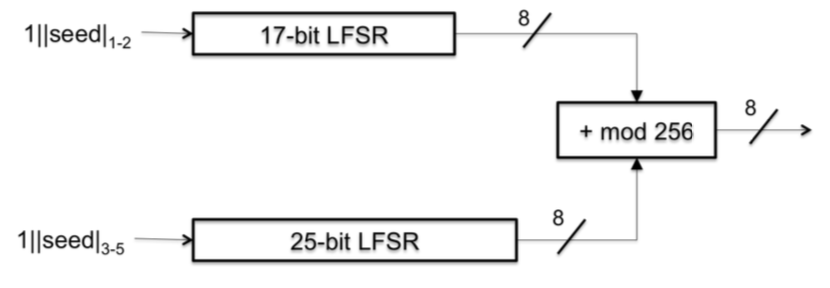
\includegraphics[width=0.5\textwidth]{img/css}
\end{figure}
\begin{itemize}
	\item $seed = key =$ 5 bytes = 40 bit 
	\item \textit{17-bit LFSR}: $1||seed[0]||seed[1]$
	\item \textit{25-bit LFSR}: $1||seed[2]||seed[3]||seed[4]$
\end{itemize}
Provare tutte le possibili chiavi: \textbf{Exaustive Key Search} ha una complessità di $O(2^{40})$ \\
L'attacco \textbf{Known-plaintext attack}, ha una complessità di $O(2^{17})$: se un avversario conosce i primi 20 bytes del plaintext e del ciphertext, può arrivare a conoscere i primi 20 bytes del keystream. Quindi, può calcolarsi il 25-bit LFSR andando a calcolare la differenza tra il seed random 17-bit LFSR e il keystream calcolato. Quindi, deve controllare se l'output 25-bit LFSR è consistente con il polinomiale, che è conosciuto.

\subsection{802.11b WEP}
\begin{itemize}
	\item pre-condivisa $k$
	\item $IV$ su $\{0,1\}^{24}$ scritto nello standard, richiesto che sia "fresco"
	\item $ks = RC4(k||iv)$, dove RC4 è il PRNG
	\item $m = m||crc(m)$
	\item $c = m \oplus ks$
\end{itemize}
Come detto, ogni volta deve essere generato un nuovo vettore di inizializzazione (IV).
Come generarlo? Con un contatore (inizializzato a zero), oppure si può generare una sequenza random con un generatore. 
Lo standard non dice nulla riguardo a come generare il vettore, dice soltanto che $sizeof(IV) = 24 bits$. 
Questo ha una forte implicazione: dopo $2^24$ frames, il vettore di inizializzazione ricomincia da capo, quindi il keystream tende ad essere ripetuto. 
Questo comportamento deve essere evitato in crittografia.
\paragraph{Drawbacks}
\begin{enumerate}[label=\alph*.]
	\item $ks$ dipende soltanto da $IV$. Come detto, dopo $2^{24}$ frames si ripete ciclicamente e $ks$ è riutilizzato.
	\item l'utilizzo di CRC, invece di una funzione hash imbrogliata da una perturbazione.
	\item utilizzo di "related keys" $k||iv, iv = 0, 1, 2, ..., 2^{24}-1$. RC4 è buono a meno che non vengano utilizzate chiavi "related".
\end{enumerate}

\section{Block ciphers}
Non lavoriamo più bit a bit, ma su blocchi di bit. Si può, in tal modo, implementare un cipher mantenendo la perfect secrecy?
La funzione E ora diventa una funzione che ha lo stesso dominio di \textit{p} ed è invertibile (mappa, quindi, ogni blocco unicamente ad un altro blocco).
Tutti i possibili blocchi di \textit{n} bit sono $2^{n}$. Per avere un cipher perfetto dobbiamo implementare tutte le permutazioni dei blocchi, da cui il numero di chiavi è uguale a $2^{n}!$.
La lunghezza in bit della chiave varia, quindi, in modo esponenziale rispetto al numero di bit per blocco (\textit{n}). \\
Tuttavia, tipicamente, n è abbastanza grande per evitare che l'avversario possa effettuare un attacco a dizionario: ciò implica che, per implementare un cifratore perfetto,
bisogna implementare un numero grande di chiavi (esponenziale). Nella pratica, quindi, non è possibile implementare la perfect secrecy nei sistemi di cifratura a blocchi. \\
Nella pratica il cipher è considerato buono se l'avversario non riesce a distinguerlo da un true block cipher. \\
Il plaintext è diviso in blocchi di lunghezza fissata $n$:

\begin{figure}[H]
  \centering
  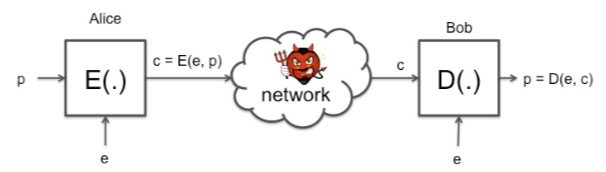
\includegraphics[width=0.5\textwidth]{img/block-cipher}
\end{figure}

\begin{itemize}
	\item $E : \{0,1\}^n \rightarrow \{0,1\}^n$
	\item $D : \{0,1\}^n \rightarrow \{0,1\}^n$
\end{itemize}
E è una \textbf{permutazione}.
Un block cipher perfetto implementa tutte le possibili permutazioni $2^{n}!$
$$\text{key size} = log_2 2^n! \approx n \times 2^n$$

The key would be too large.
In practice, the encryption function corresponding to a randomly chosen key ($E(k, x)$) should appear as a randomly chosen permutation ($\pi(x)$).

\begin{figure}[H]
  \centering
  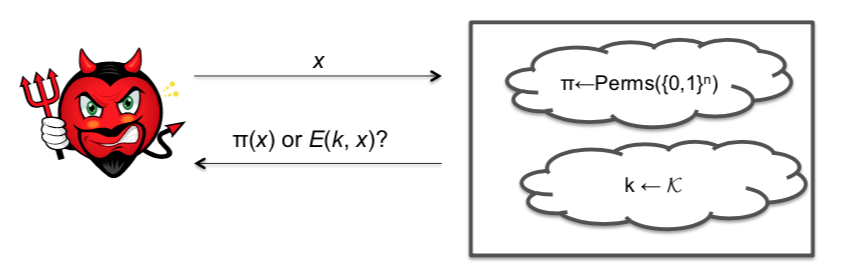
\includegraphics[width=0.5\textwidth]{img/perm}
\end{figure}

The block size should be large enough to make the dictionary attack unfeasible in terms of storage complexity, i.e. if $n = 64$, and adversary should store $2^{64} \times (8 \times 2)$ bytes (8 bytes for plaintext and ciphertext).

\subsection{DES improvements}
DES is deprecated because of the shortness of the key (56 bits).

\subsubsection{2DES}

\begin{figure}[H]
  \centering
  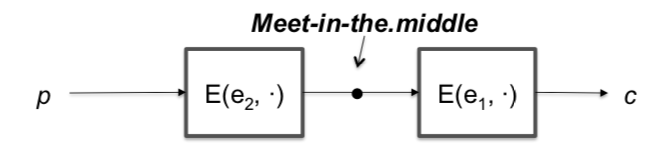
\includegraphics[width=0.5\textwidth]{img/2des}
\end{figure}

$$k = k_1 + k_2$$

Even if the new key is on 112 bits, it does not improve the security because the MITM attack (KPT attack) has complexity of $O(2^{56})$ to find $k_1$ and $O(2^{56})$ to find $k_2$ comparing the encrypted text $X_L$ and the decrypted one $Y_L$. This leads to a total complexity of $O(2^{56})$. Furthermore, it halves the performance.

\subsubsection{3DES}

\begin{figure}[H]
  \centering
  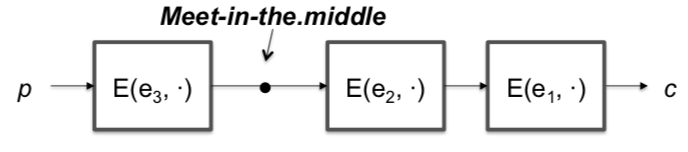
\includegraphics[width=0.5\textwidth]{img/3des}
\end{figure}

$$k = k_1 + k_2 + k_3$$

The new key is on 168 bits and the MITM attack has a complexity of $O(2^{56\times2}) = O(2^{112})$.
In $EDE$ version $k_1 = k_2 = k_3$.

\subsubsection{Key whitening}
It is used in strong "black box" (without internal vulberability) ciphers which use short keys.

It foresees only one encryption process plus pre-xor and post-xor:
$$ c = k_2 \oplus E(k, (m \oplus k1)) $$

\paragraph{Attacks complexity}
\begin{itemize}
	\item bruteforce attack: $O(2^{k+2n})$ computational
	\item MITM attack: $O(2^{k+n})$ computational + storage
	\item most efficient attack: the adversary knows $2^m$ (PT-CT)-pairs (data complexity) $\Rightarrow$ $O(2^{k+n-m})$
\end{itemize}

\section{Exhaustive key search}
With $k > n$ it is possible to find false positive keys. Given a pair $x_1$ and $y_1$, the probability that key $k$ is able to map $x_1$ in $y_1$ is:
$$ P = \frac{1}{2^n} $$
because the algorithm can be considered secure and the ouput can be seen as an uniform random variable.

Since the number of keys are $2^k$, the number of expected candidate keys is:
$$ E(\#keys) = 2^k \times \frac{1}{2^n} = 2^{k-n}$$
If I want to reduce the set of candidate keys I have to collect other pairs (related to the concept of \textit{unicity distance}). If I have $t$ plaintext-ciphertext pairs, the number of expected candidate keys will be:
$$ E(\#keys) = 2^{k-tn} $$
A multiple encryption with r-stage of encryption has $2^{rk-tn}$ candidate keys.

\section{Confusion and diffusion}
According to Shannon, there are two primitive operations with which strong encryption algorithms can be built:
\begin{itemize}
	\item \textbf{Confusion}: relationship between key and ciphertext is obscured using substitution
	\item \textbf{Diffusion}: the influence of one plaintext symbol is spread over many ciphertext symbols with the goal of hiding statistical properties of the plaintext using permutation
\end{itemize}
These two operations must be concateneted.

\section{Data Encryption Standard (DES)}
\begin{itemize}
	\item $n = 64$
	\item $k = 56$
\end{itemize}
DES is an iterative algorithm. For each block of plaintext, encryption is handled in 16 rounds which all perform the identical operation. In every round a different subkey is used and all subkeys $k_i$ are derived from the main key $k$ by the \textit{key schedule}.

\begin{figure}[H]
  \centering
  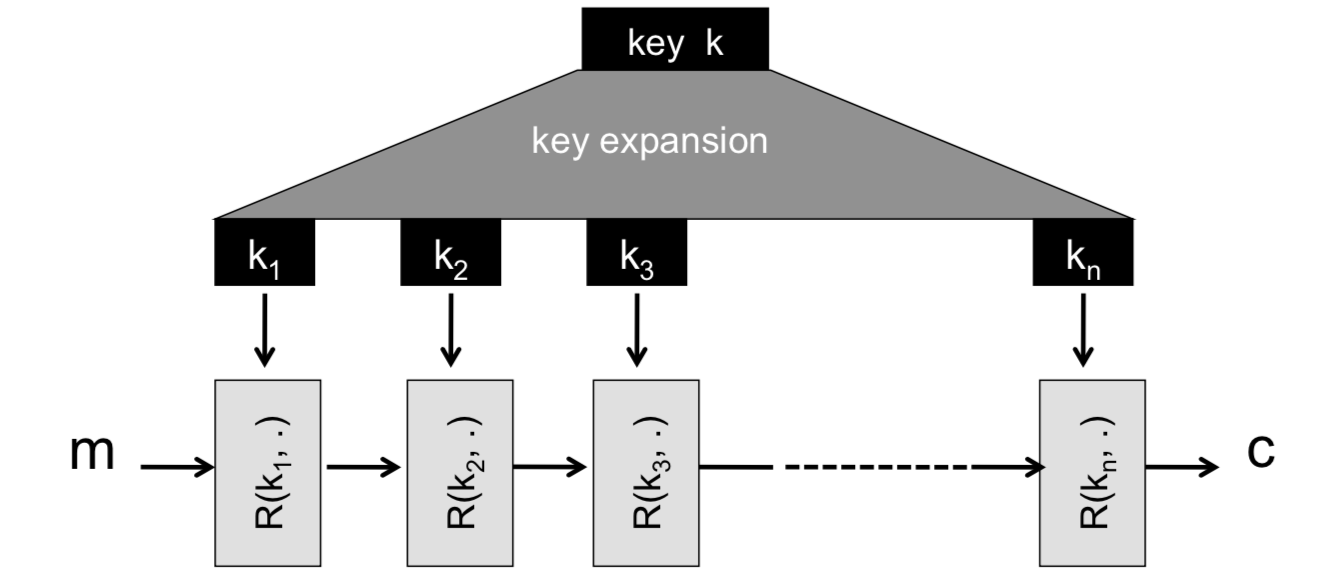
\includegraphics[width=0.5\textwidth]{img/key-schedule}
\end{figure}

The round function is built by means of a \textit{Feistel network}:

\begin{figure}[H]
  \centering
  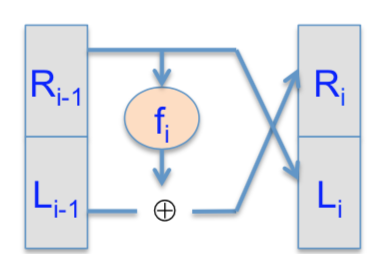
\includegraphics[width=0.2\textwidth]{img/feistel}
\end{figure}

\begin{align}
&L_i = R_{i-1} \notag\\
&R_i = L_{i-1} \oplus f(R_{i-1}, k_i) \notag
\end{align}

One advantage of Feistel networks is that encryption and decryption are almost the same operation, just traversing the network in the opposite direction uning keys in reverse order.

\begin{align}
&R_{i-1} = L_i \notag\\
&L_{i-1} = R_i \oplus f(R_{i-1}, k_i) = R_i \oplus f(L_i, k_i) \notag
\end{align}

Feistel structure really only encrypts (decrypts) half of the input bits per each round.

\subsection{Round function \textit{f}}

\begin{figure}[H]
  \centering
  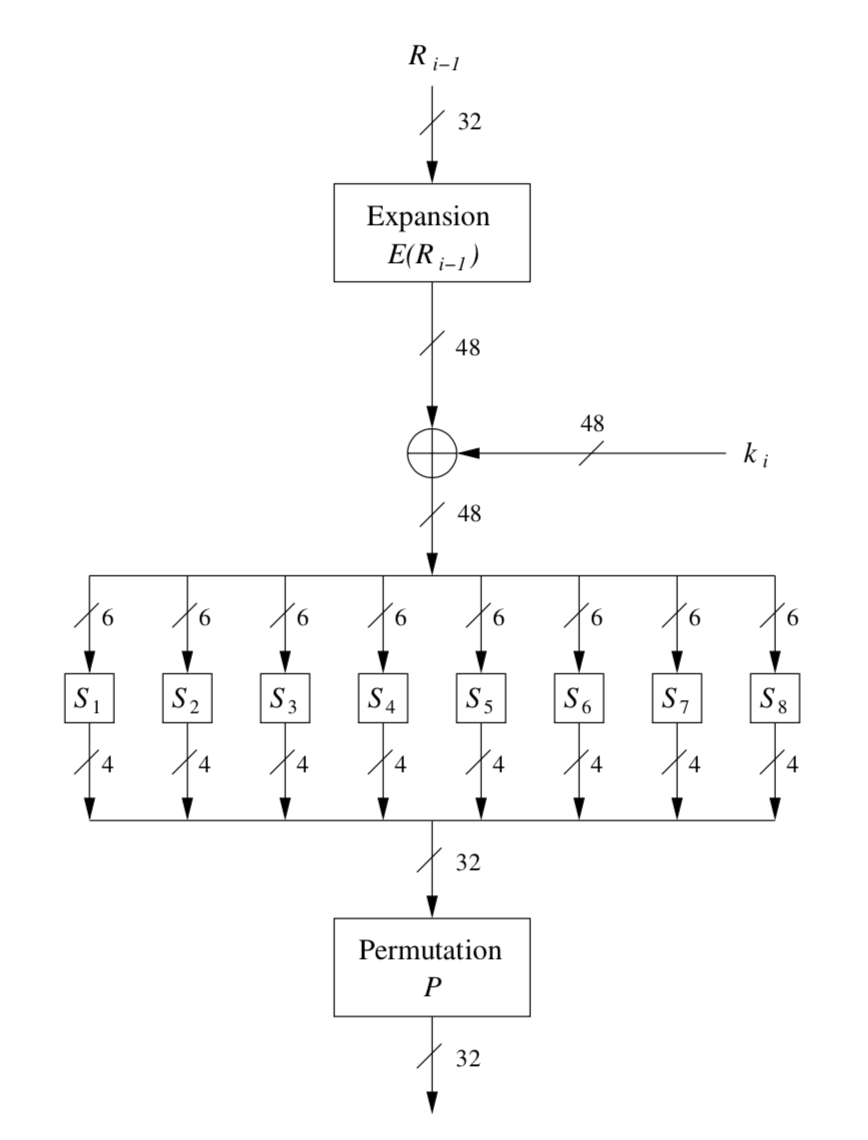
\includegraphics[width=0.5\textwidth]{img/round-func}
\end{figure}

The $f$ function is a pseudo-random generator with the two input parameters $R_{i-1}$ and $k_i$. It should be unpredictable. It uses nonlinear building blocks and maps 32 input bits to 32 output bits using a 48-bit round key $k_i$, with $1 \leq i \leq 16$.

\textit{Diffusion} is done on by \textit{initial permutation IP} using bytewise permutation and duplication, \textit{confusion} is made by S-boxes.

\subsection{DES properties}
DES, as a good cipher, fullfills the following properties:
\begin{itemize}
	\item each ciphertext bit depends on all key and plaintext bits
	\item there are not any evident statistical relationship between the plaintext and the ciphertext
	\item the change of one bit in the plaintext (ciphertext) causes the change of the every bit in the ciphertext (plaintext) with 0.5 probability (uniform RV).
\end{itemize} 

\section{Encryption Modes}
\subsection{Electronic Codebook (ECB)}
\begin{figure}[H]
  \centering
  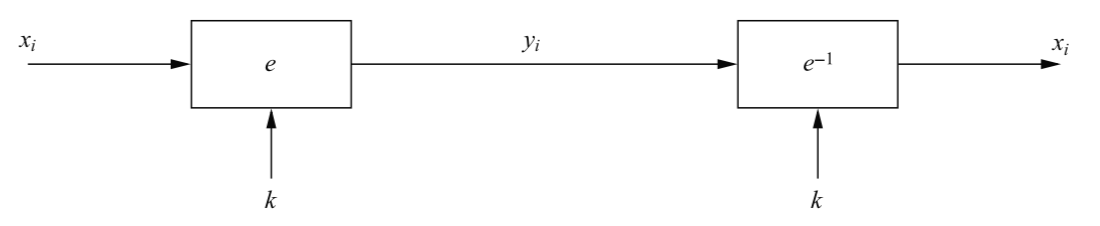
\includegraphics[width=0.5\textwidth]{img/ecb}
\end{figure}
\paragraph{Pros}
\begin{itemize}
	\item No block synchronization is required
	\item No error propagation
	\item Can be parallelized
\end{itemize}
\paragraph{Cons}
\begin{itemize}
	\item Identical plaintext block results in identical ciphertext block: it does not hide data pattern and allows traffic analysis
	\item it allows block re-ordering and substitution
\end{itemize}

\subsection{Cipherblock Chaining (CBC)}
\begin{figure}[H]
  \centering
  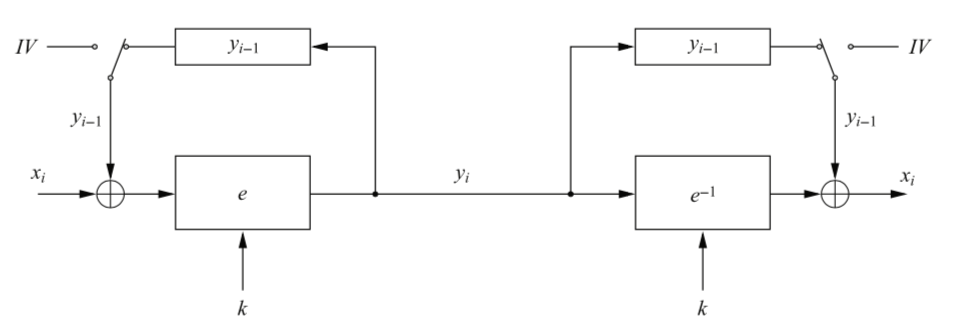
\includegraphics[width=0.5\textwidth]{img/cbc}
\end{figure}
CBC suffers form error propagation.

\subsection{Cipher Feedback (CFB)}
\begin{figure}[H]
  \centering
  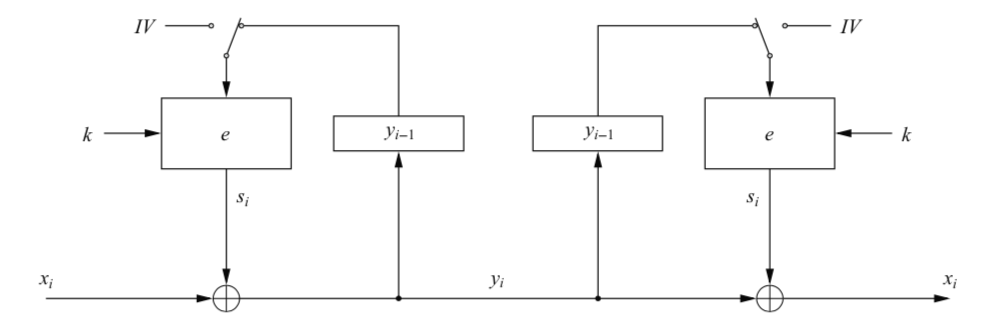
\includegraphics[width=0.5\textwidth]{img/cfb}
\end{figure}
CFB is an asynchronous blockwise stream cipher becasue it depends on the previous ciphertext.

\subsection{Output Feedback (OFB)}
\begin{figure}[H]
  \centering
  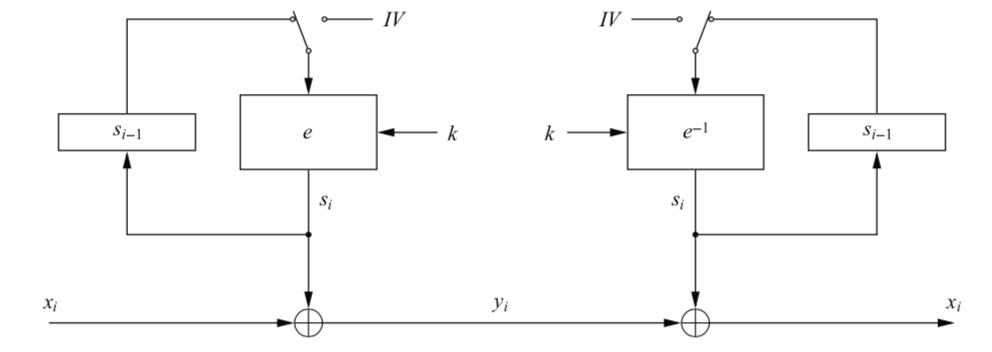
\includegraphics[width=0.5\textwidth]{img/ofb}
\end{figure}
OFB is a synchronous blockwise stream cipher and it allows pre-computation because the next block does not depend on netiher $PT$ or $CT$.

\subsection{Counter Mode (CTR)}
\begin{figure}[H]
  \centering
  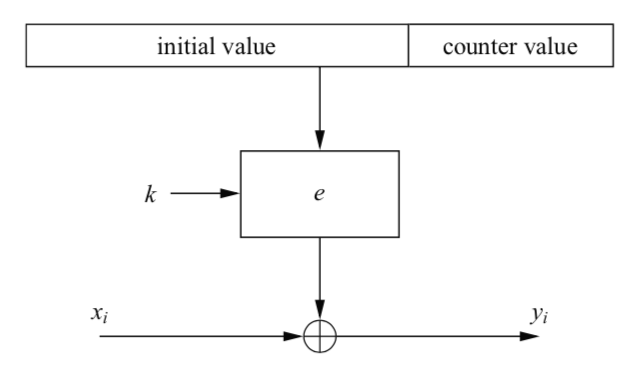
\includegraphics[width=0.3\textwidth]{img/ctr}
\end{figure}
It gives an upper limit to the amount of data that can be encrypted.

\section{Padding (PKCS \#7)}
Padding is used to make the plaintext length multiple of block size $n$. In all cases the ciphertext length is always greater than the plaintext. This phenomenon is called \textit{ciphertext expansion}.

\subsection{Ciphertext Stealing Mode (CTS)}
It encrypts using ECB without ciphertext expansion.

\begin{figure}[H]
  \centering
  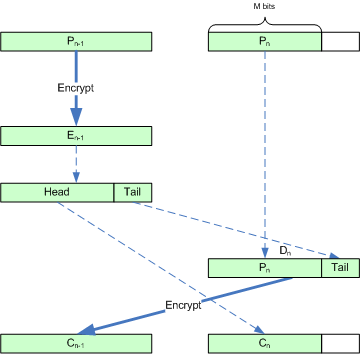
\includegraphics[width=0.3\textwidth]{img/cts}
\end{figure}


\section{Advanced Encryption Standard (AES)}
\begin{itemize}
	\item $n = 128$
	\item $k = 128/192/256$
\end{itemize}

\begin{center}
\begin{tabular}{ c | c }
key lengths & \# rounds = $n_r$ \\
\hline
128 bit & 10 \\ 
192 bit & 12 \\  
256 bit & 14    
\end{tabular}
\end{center}

AES does not have a Feistel structure. 

\begin{figure}[H]
  \centering
  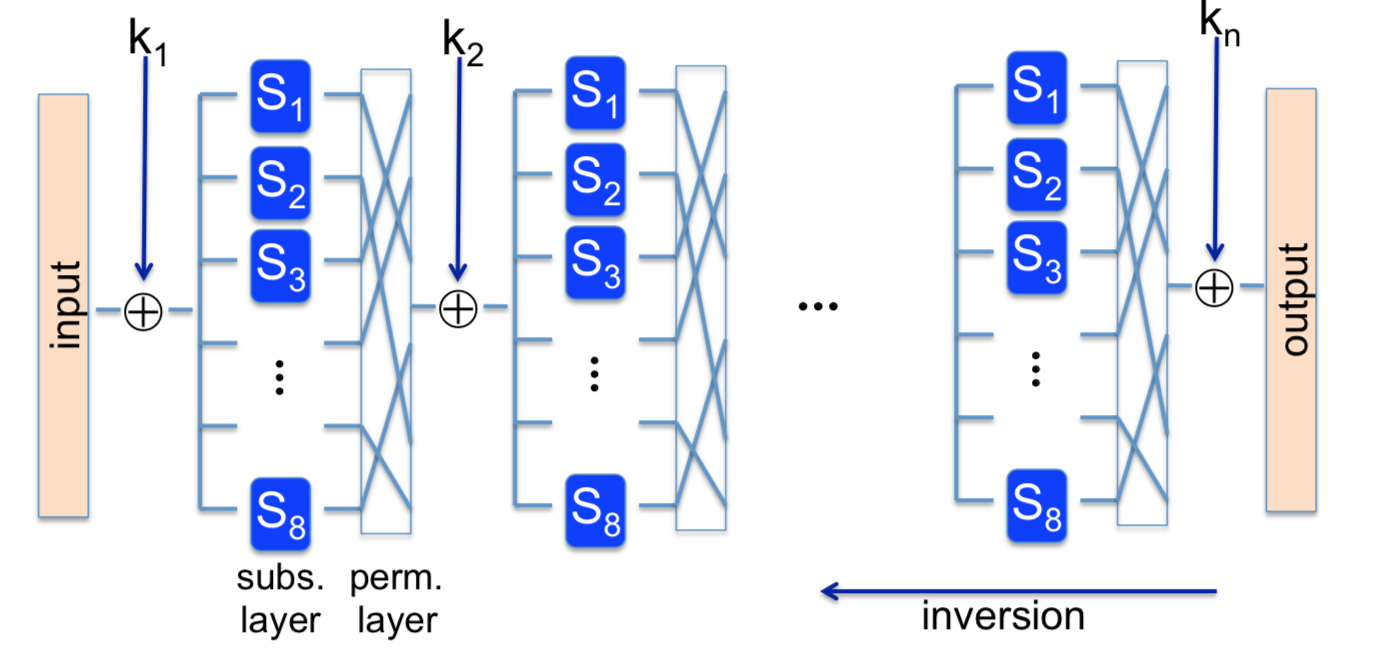
\includegraphics[width=0.5\textwidth]{img/aes}
\end{figure}

AES consists of three \textit{layers}:
\paragraph{Key addition layer} A 128-bit round key which has been derived from the main key in the key schedule, is XORed to the state
\paragraph{Byte substitution layer (S-box)} It introduces \textit{confusion} by transforming nonlinearly each elemeny of the state using lookup tables
\paragraph{Diffusion layer} It introduces \textit{diffusion} through the following operations: \textit{ShiftRows} and \textit{MixColumn}.

\section{Hash function}
It provides message integrity.
$$ H : \{0,1\}^* \rightarrow \{0,1\}^n $$
Collision occurs when at least two inputs have the same \textit{digest}.

A secure hash function is when collisions exist but they are "difficult" to find.

\subsection{Security properties}
\paragraph{Preimage resistance or One-Wayness}
Given a hash output $z$ it must be "difficult" to find the input $x$ such that $z = h(x)$
\paragraph{Second Preimage Resistance or Weak Collision Resistance}
Given an input $x$ it must be "difficult" to find $x'$ such that $h(x) = h(x')$
\paragraph{Collision Resistance}
It must be "difficult" to find $x$ and $x'$ such that $h(x) = h(x')$

\subsection{Black box attacks}
These attacks do not exploit the internals of the hash function:
\begin{itemize}
	\item Guessing attack against $2^{nd}$ preimage: $O(2^n)$
	\item Birthday attack against $3^{rd}$ preimage: $O(2^{\frac{n}{2}})$
\end{itemize}

\subsection{Merkle-Damgard scheme}
This scheme is used to build the hash function H. If we want to build a Collision Resistant Hash Function (CRHF) we need a collision resistant $h$.

\subsubsection{Davies-Meyer scheme}
\begin{figure}[H]
  \centering
  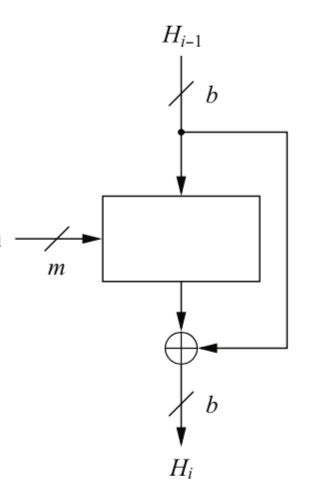
\includegraphics[width=0.2\textwidth]{img/davies-meyer}
\end{figure}
This scheme is used to build a collision resistant $h$. It is build using a block cipher (i.e. AES-128) which takes $H_i$ as input and $x_i$ as key.
The final output is obtained by XOR operation which makes $h$ collision resistant:
$$ H_{i+1} = E(x_i, H_i) \oplus H_i $$ 

To make the birthday attack much more unfeasible the \textit{Hirose scheme} can be used. Indeed it foresees the use of two block ciphers in order to have an output of $2\times128$ bit.

\section{Message Authentication Codes (MACs)}
It provides message integrity and message authentication.

\begin{figure}[H]
  \centering
  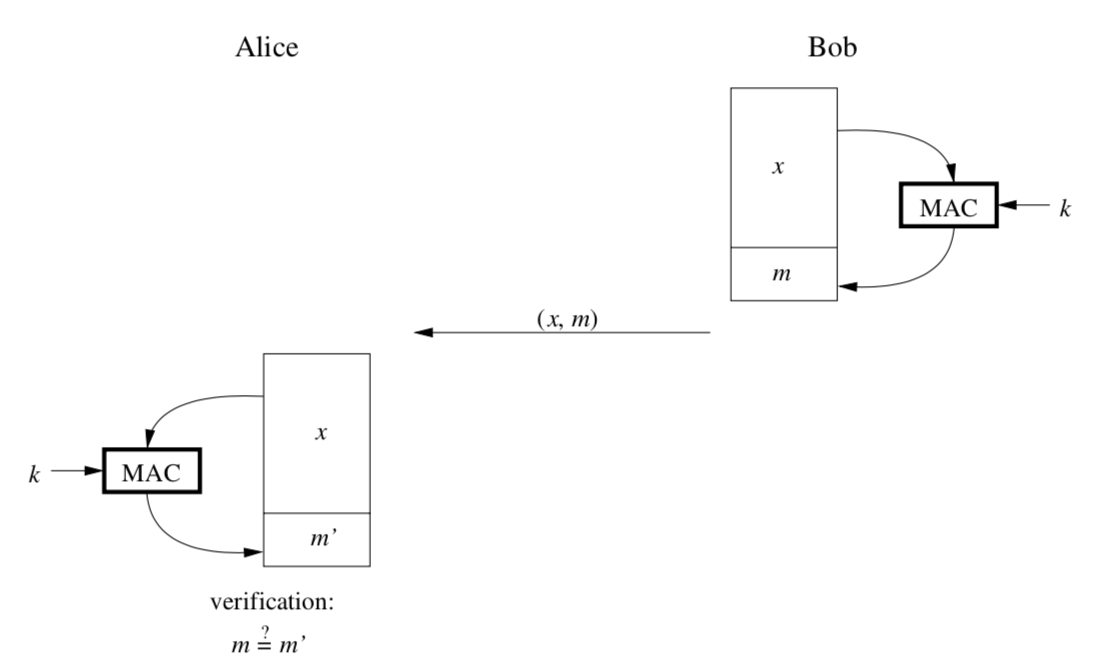
\includegraphics[width=0.5\textwidth]{img/mac}
\end{figure}

\begin{itemize}
	\item $m$: clear message
	\item $k$: shared key between the two parties
	\item $t$: tag or digest or fingerprint
	\item $S$: MAC generation algorithm
	\item $V$: MAC verification algorithm
\end{itemize}

\subsection{MAC generation algorithm}
\begin{itemize}
	\item It must be "easy"
	\item $S : \{0,1\}^* \rightarrow \{0,1\}^n$ is an hash function
	\item \textbf{Computational resistance property} (\textit{key non-recovery}): for a certain key $k$, given ($m_i, t_i$), where $t_i = S(k, m_i)$, it must be "difficult" to compute $(m, t) : t = S(k, m)$ for any $m \neq m_i$ without knowing $k$.
\end{itemize}

MACs do not provide no-repudiation.

\subsection{MACs from hash function}
\paragraph{Secret prefix scheme} 
$$t = h(k||m)$$
It is not secure because the MAC can be constructed from $m$ without knowing the key.

\paragraph{Secret postfix scheme}
$$t = h(m||k)$$
If an adversary finds a collision in the hash function, i.e. $m_0 : h(m) = h(m_0)$, then $$h(m||k) = h(m_0||k)$$.

\paragraph{HMAC}
$$ t = h[(k \oplus opad) || h[(k \oplus ipad) || m]]$$
where $opad, ipad$ are fixed known seqence of bit specified in the standard.

\subsection{MACs from block ciphers: CBC-MAC}
\begin{figure}[H]
  \centering
  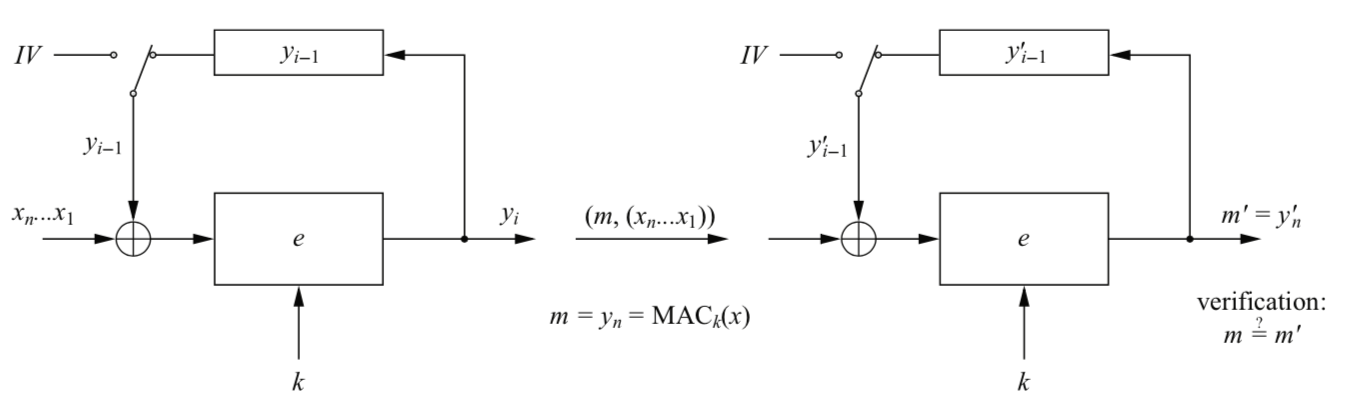
\includegraphics[width=0.5\textwidth]{img/cbc-mac}
\end{figure}
The problem of this scheme is that an adversary can create another pair $(m,t)$ without knowing the key if the message size is just one block.
It just needs to append $m \oplus t$ to the original message $m$ so that the last encryption produces the same digest with $m' = m||(m \oplus t)$:
$$ E_k(t \oplus (m \oplus t)) = t $$

\section{Key establishment}
\subsection{Diffie-Hellman}
This protocol allows to share the session key without a pre-shared key.
\begin{itemize}
	\item $p$ is a large (2048 bit) prime number
	\item generator $g : \forall y, 1 \leq y < p, \exists x : y = g^x\ mod\ p$
\end{itemize}
Either $p$ and $g$ are public. Each peer generates the private key and computes the public key out of it. The session key will be:
$$ k_{ab} = g^{ab}\ mod\ p $$

\paragraph{Discrete exponentiation}
Given $p$, $g$ and $x$, to compute $y = g^x\ mod\ p$ is computationally easy.

\paragraph{Discrete logarithm}
Given $g$, $1 \leq y \leq p-1$, it is computationally difficult to determine $x, 1 \leq x \leq p-1 : y = g^x\ mod\ p$.

\subsubsection{Passive attack}
For a passive attack DH is secure: a passive adversary can only see $Y = g^x\ mod\ p$. In order to get the key $x$ it must solve the \textit{discrete logarithm} problem which is "difficult".

\subsubsection{Active attack}
A MITM attack can break DH. An adversary can establish a session key with both parties and act as a valid party. There is nothing that links the public key $Y$ to an identifier.

\section{Public key encryption}
It is an asymmetric encryption and it needs a generator $G$ that is able to generate random quantities which correspond to the private and public keys.

Public cryptography is used for key establishment.

\subsection{Security properties}
\begin{itemize}
	\item Given $pubk$ and $y$ it must be "difficult" to find $x : E(pubk, x) = y$
	\item Known $pubk$ it must be "difficult" to find $privk$
\end{itemize}

There not exists any perfect public key cipher:
\begin{enumerate}
	\item Intercept $y$
	\item Select $x_0 : P(X = x_0) \neq 0$
	\item Compute $y_0 = E(pubk, x_0)$
	\item \texttt{if} $y == y_0$ $x$ is found \texttt{else} $P(X=x_0|Y=y) = 0$
\end{enumerate}

The \textit{a-priori} and \textit{a-posteriori} probabilities are different and violate the Shannon's definition of perfect secrecy.

\section{RSA}
\subsection{Key generation algorithm G}
\begin{enumerate}
	\item Select "large" (512/1024 bit) primes $p$ and $q$
	\item Compute \textit{modulus} $n = p \cdot q$ and \textit{Eulero's totient} $\Phi = (p-1)\cdot(q-1)$
	\item Compute $1 \leq e < \Phi : g.c.d(e, \Phi) = 1$ ($e$ and $\Phi$ comprimes)
	\item Compute $1 \leq d < \Phi : e\cdot d = 1\ mod\ \Phi$, i.e. $e\cdot d = r\cdot\Phi + 1$ for some $r$
	\item $pubk = (e,n)$ and $privk = (d,n)$
	\item Destroy $p$ and $q$
\end{enumerate}

\subsection{Encryption}
$$ x \in [0, n-1], y = x^e\ mod\ n$$

\subsection{Decryption}
$$ y \in [0, n-1], x = y^d\ mod\ n$$

\subsection{Square-and-multiply algorithm}
This algorithm is used to perform the modular exponentiation $x^e\ mod\ n$ with a complexity of $O(k^3)$.

\begin{algorithm}[H]
\begin{algorithmic}
\State $c \gets 1$
\ForAll{bit in e} 
	\State $c \gets c^2\ mod\ n$
	\If{bit == 1} \State $c \gets c \times x\ mod\ n$ \EndIf

\EndFor
\end{algorithmic}
\end{algorithm}


Efficiency is achieved choosing $e$ with few bit equal to 1, i.e. $2^{16} + 1$.

\subsection{RSA problem}
The computation of $x$, knowing $(e,n)$ and $y$, is related to the \textit{factorization} problem.

Computing the decryption exponent $d$ from the public key $(e, n)$ is computationally equivalent to factoring $n$.

\subsection{RSA security}
\subsubsection{Small plaintext problem}
If the plaintext is too small the resulting ciphertext is equal to the plaintext.

\subsubsection{Malleability}
An adversary knows $c = p^e\ mod\ n$ and it can compute
$$ c' = c \cdot s^e\ mod\ n = p^e \cdot s^e\ mod\ n = (p \cdot s)^e\ mod\ n = p'\ mod\ n $$
where $s$ is an integer such that $g.d.c(s, n) = 1$.

\subsubsection{Low exponent attack}
Let $e = 3$ so that $c_i = m^3\ mod\ n_i$.
A party sends $c$ to three different receivers which compute $m^3 = c_i\ mod\ n_i$.
If $n_1, n_2, n_3$ are pairwise comprime we can compute 
$$ x = m^3\ mod\ n_1n_2n_3$$ 
using \textit{Chinese Remainder Theorem} (CRT).

Since $m^3 < n_1n_2n_3$, $x = m^3$. So an adversary compute $m$ by computing the cube root of $m^3$.

\subsubsection{Common modulus attack}

\begin{figure}[H]
  \centering
  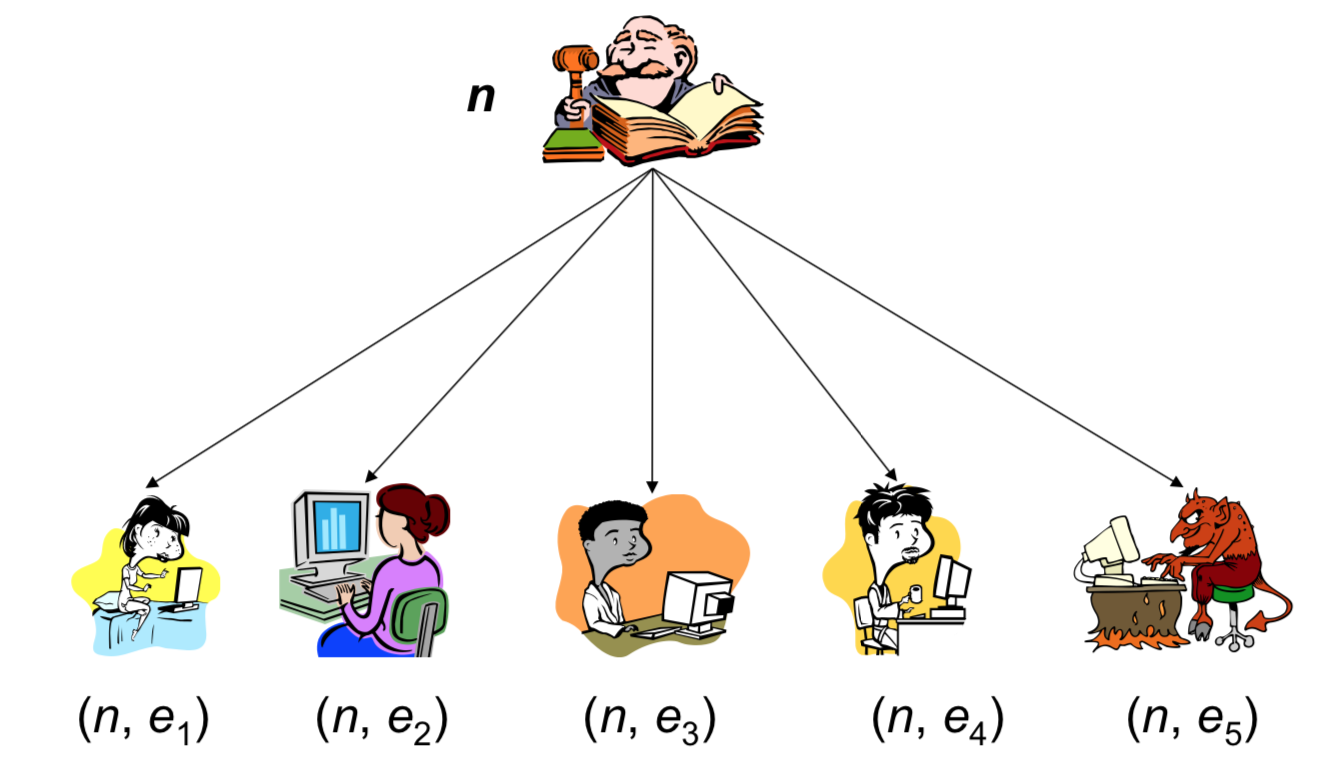
\includegraphics[width=0.5\textwidth]{img/common-modulus-attack}
\end{figure}

The attacker can efficiently factor $n$ from $d_5$ and then compute all $d_i$.

\subsubsection{Chosen-plaintext attack}

\begin{figure}[H]
  \centering
  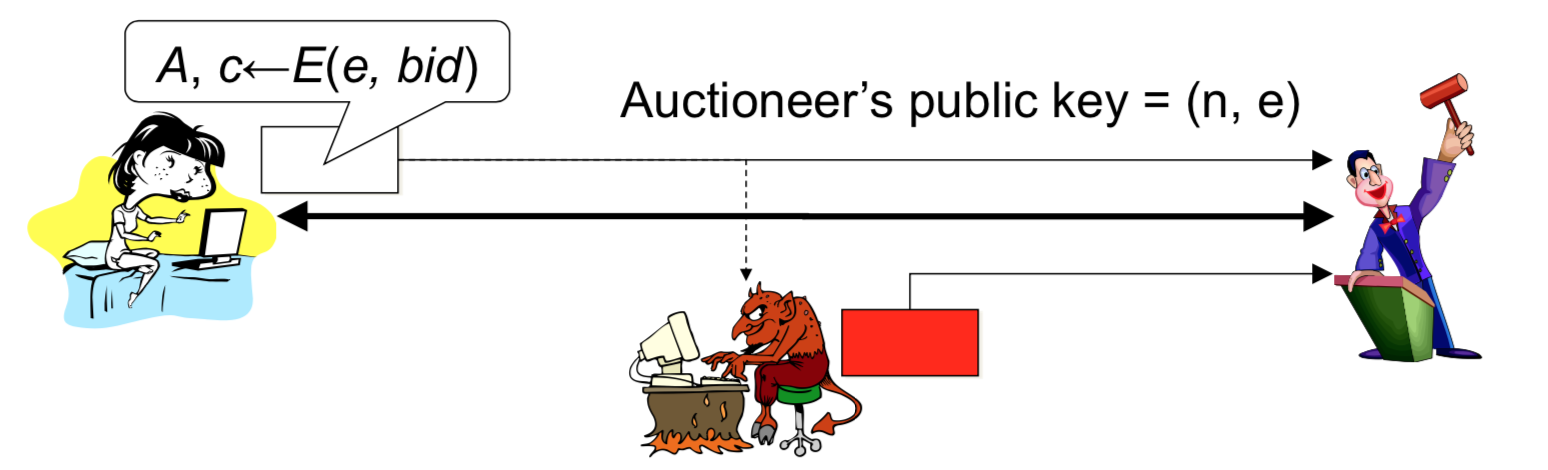
\includegraphics[width=0.5\textwidth]{img/chosen-plaintext-attack}
\end{figure}

The adversary encrypts all possible bids (e.g, $2^{32}$) until he finds a $b$ such that $E(e, b) = c$. Thus, the adversary sends a bid containing the minimal offer to win the auction: $b' = b + 1$.

\subsubsection{Adaptive chosen-plaintext attack}

\begin{figure}[H]
  \centering
  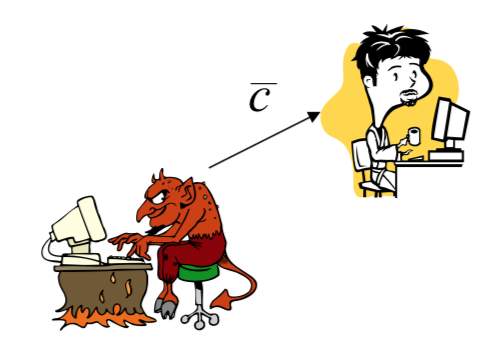
\includegraphics[width=0.3\textwidth]{img/chosen-ciphertext-attack}
\end{figure}

Bob decrypts ciphertext except a given ciphertext $c$. Mr. Loucipher wants to determine the ciphertext corresponding to $c$.

\begin{enumerate}
	\item Mr. Loucipher selects $x$ at random, such that $gcd(x, n) = 1$, and sends Bob the quantity $\overline{c} = cx^e\ mod\ n$;
	\item Bob decrypts it producing $\overline{m} = (\overline{c})^d = c^d x^{ed} = mx\ mod\ n$;
	\item Mr. Loucipher determines $m$ by computing $m = \overline{m} x^{-1}\ mod\ n$.
\end{enumerate} 

\subsubsection{Countermeasure}
Add redundancy and randomization to the original message through \textit{Optimal Asymmetric Encryption Padding} standard.

\section{Digital signature}
DS provides message integrity and message authenitication like MACs but using asymmetric key environment. Moreover, it gurantees non-repudiation property because only one party has the private key.

Anyone can verify the signature.

DS can be made by using RSA:
\begin{enumerate}
	\item Generate RSA key pair: public key $(e,n)$ and private key $(d,n)$
	\item Sign: $\sigma = m^d\ mod\ n$
	\item Verification: $m' = \sigma^e\ mod\ n$ and check if $m == m'$
\end{enumerate}

\subsection{Properties from hash function}
\paragraph{Pre-image resistance}
Let $\sigma = h(m)^d\ mod\ n$. If $h$ is not pre-image resistant:
\begin{enumerate}
	\item Select $z < n$
	\item Compute $y = z^e\ mod\ n$
	\item Find $m' : h(m') = y$
	\item Claims that $z$ is the digital signature of $m'$
\end{enumerate}

\paragraph{Second pre-image resistance}
Let $\sigma = h(x)^d\ mod\ n$ a digital signature of Alice. If $h$ is not 2nd-preimage resistance an adversary can claim that Alice has signed $x'$ instead of $x$.

\paragraph{Collision resistance}
If $h$ is not collision resistance an untrusted party can:
\begin{enumerate}
	\item Choose $m, m' : h(m) = h(m')$
	\item Produce $\sigma = h(m)^d\ mod\ n$
	\item Send $(m, \sigma)$ to Bob
	\item Then claim that it actually issued $(m', \sigma)$
\end{enumerate}

\section{Certifiate}
A certificate links the identifier to the public key.
$$ CERT_A = (Alice, pubkey_A, L_A, S_{CA}(Alice, pubkey_A, L_A))$$

\subsection{Diffie-Hellman MITM solution}

\begin{figure}[H]
  \centering
  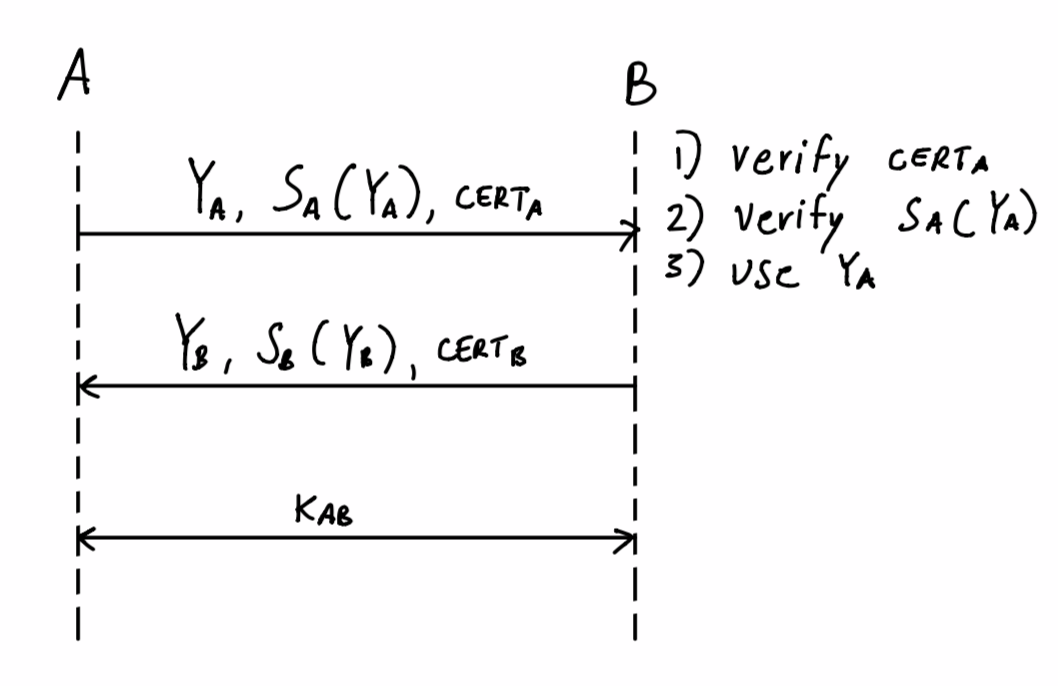
\includegraphics[width=0.5\textwidth]{img/dh-cert}
\end{figure}

\subsection{CA delegation}
If Bob wants to sign certificates, he must have a certificate like this:
$$ CERT_B = S_{CA}(Bob, pubkey_B, ..., "CA:yes")$$

\subsection{Certificate revocation}
All the revoked certificates are listed in the \textit{Certificate Revocation List} (CRL) with the relative fields all signed by CA:
\begin{itemize}
	\item serial number
	\item revocation date
	\item revocation reason
\end{itemize}

\subsection{Private key backup: Threshold Crypto}
The idea is to split the private key into $n$ shares stored in $n$ different servers.
For reconstructing the key, only $t : t < n$ shares are needed using, for instance, a linear polynomial algorithm.

\section{Perfect Forward Secrecy (PFS)}
DEF: Disclosure of long-term secret keying material does not compromise the secrecy of the exchanged keys from earlier runs.

\subsection{Pre-Shared Key Ephemeral DH}
Pre-shared key is used for authentication.
Key $a$ and $b$ are ephemeral because they are used one time per session or message.

\begin{figure}[H]
  \centering
  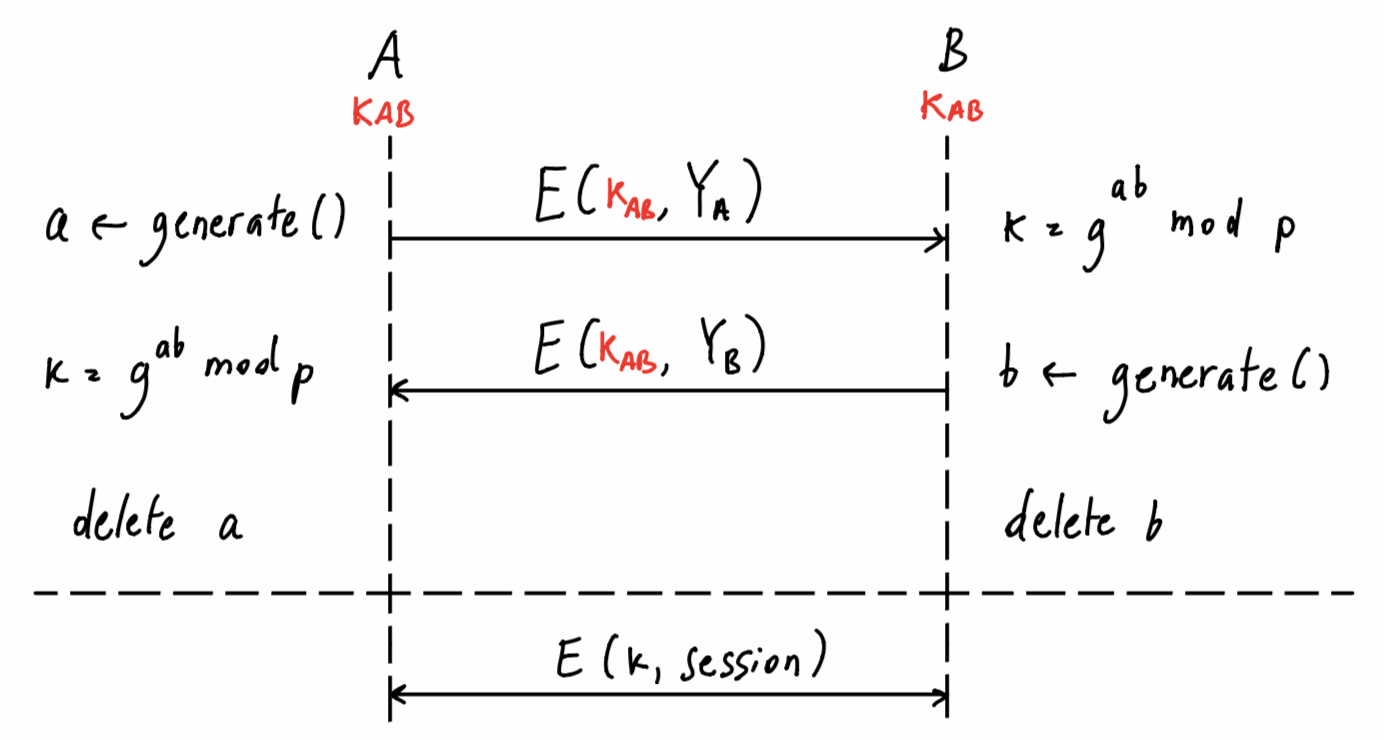
\includegraphics[width=0.5\textwidth]{img/psk-dhe}
\end{figure}

\subsection{Ephemeral RSA}
Private key is used for authentication.
B generates $Tpubk$ and $Tprivk$ on the fly used to exchange the session key.

\begin{figure}[H]
  \centering
  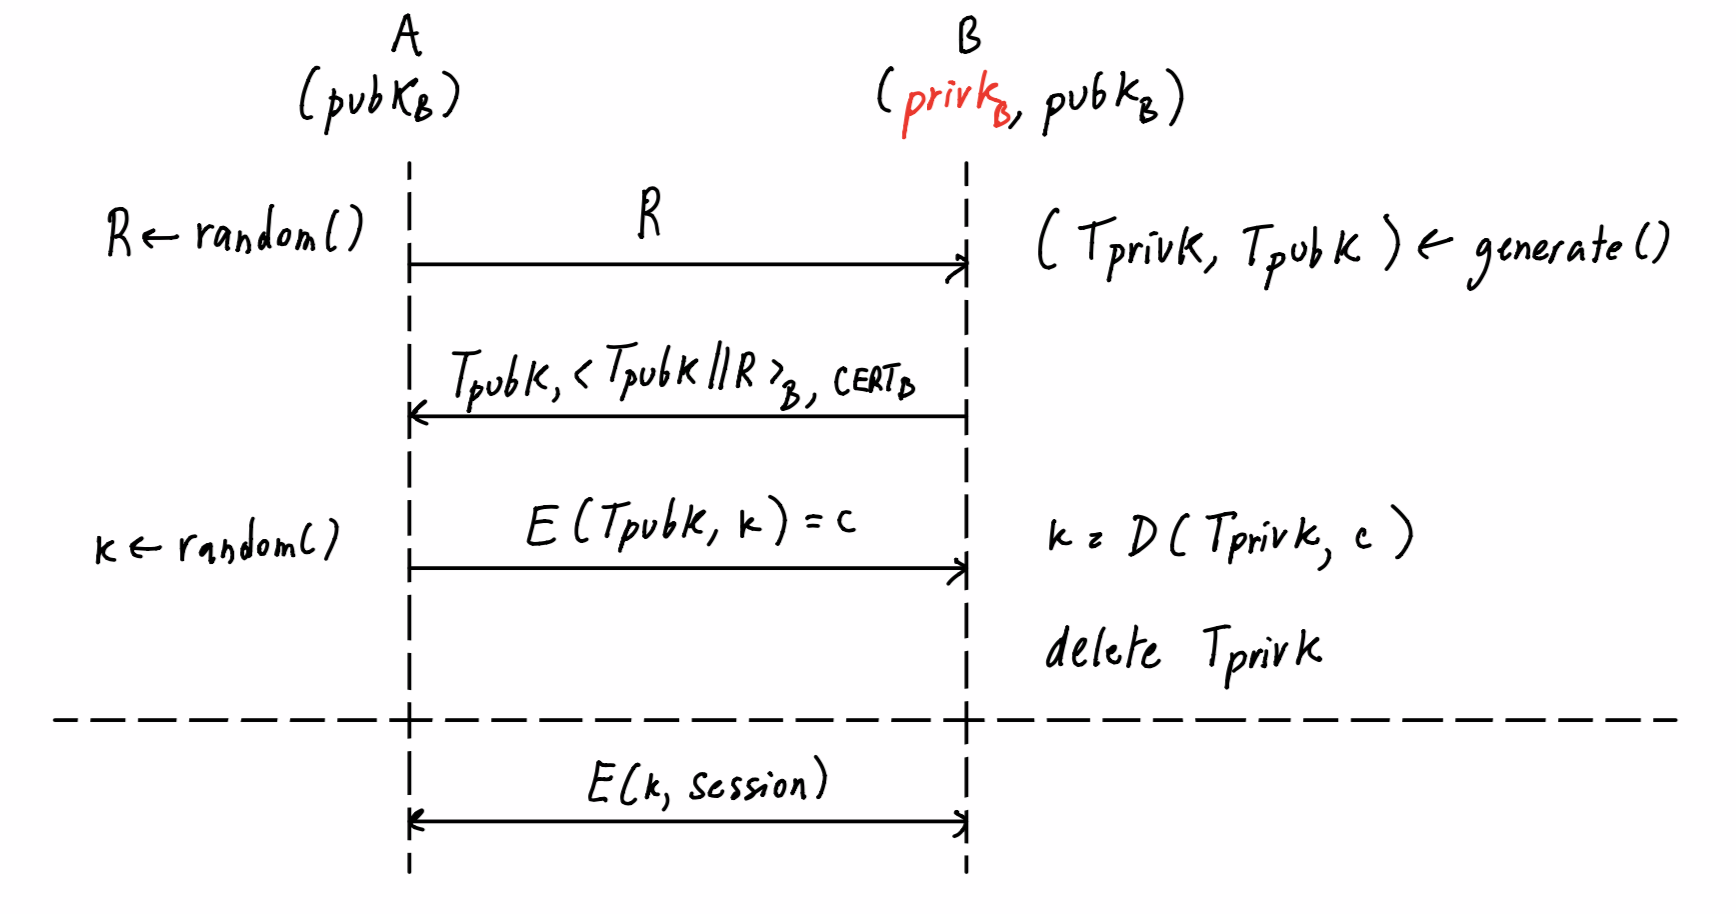
\includegraphics[width=0.5\textwidth]{img/rsae}
\end{figure}

Note that A, at the end of the key exchange phase, has not any guarantees that B has the key in its hands.

\subsection{Station-To-Station (STS) protocol}
It guarantees PFS and direct authentication (or key confirmation).

\begin{figure}[H]
  \centering
  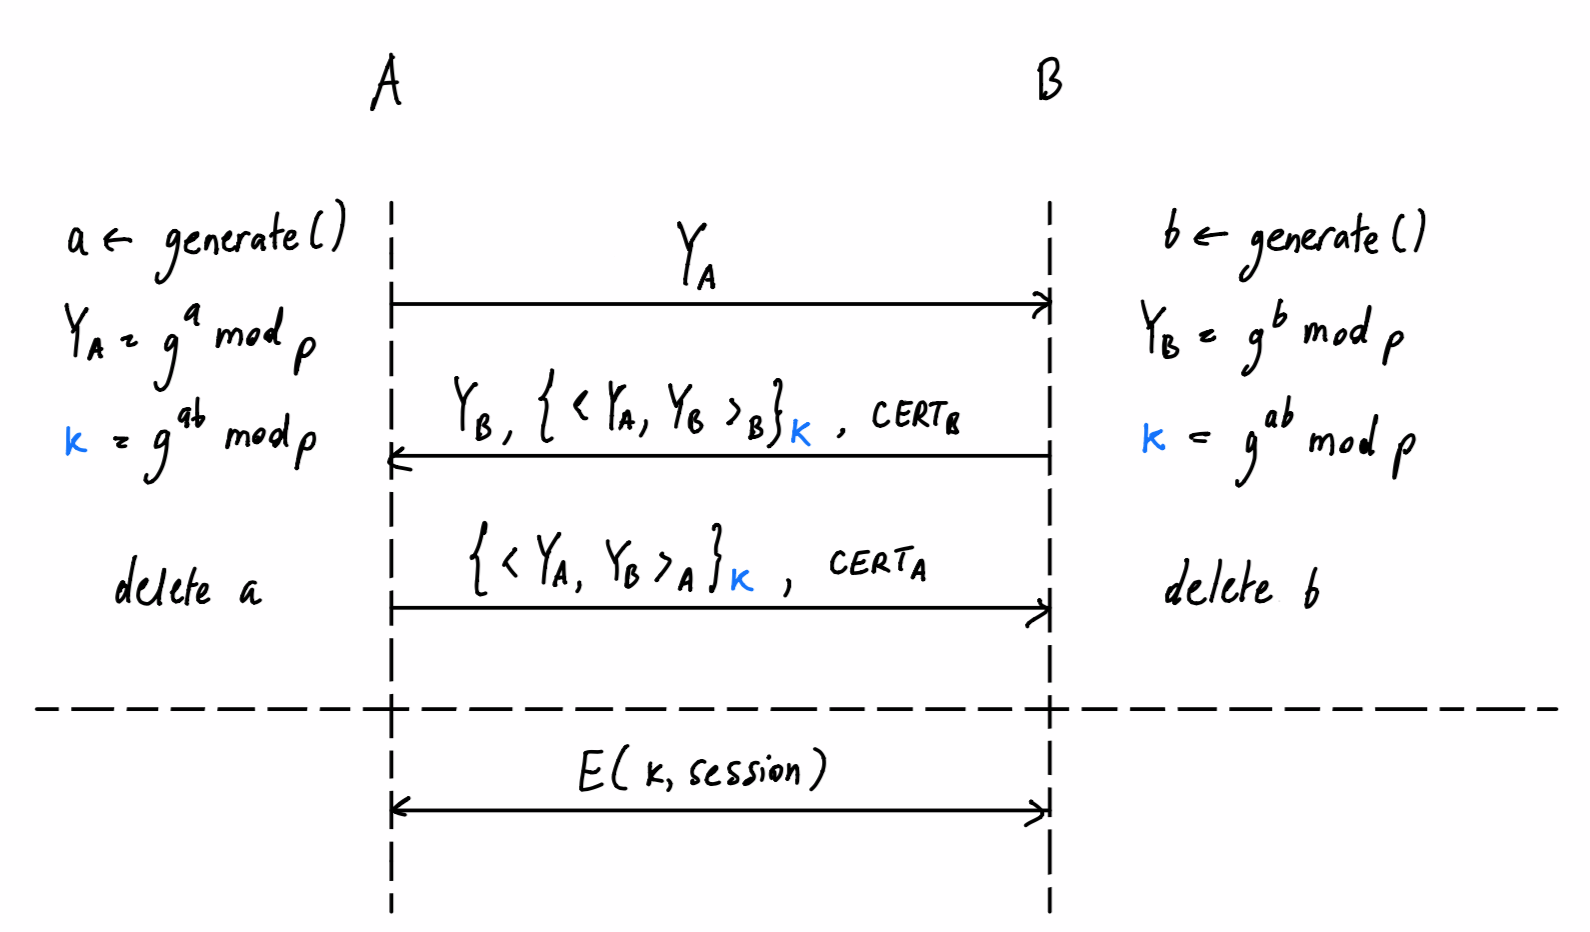
\includegraphics[width=0.5\textwidth]{img/sts}
\end{figure}

The pair $<Y_A,Y_B>$ is signed in order to avoid MITM attack. The encryption by means of $k$ is done just to guarantee \textit{direct authentication}.

\section{BAN logic}
\subsection{Postulate 1: message meaning rule}

\[\frac{P \believes Q \sharekey{k} P, P \sees \encrypt{X}{k}}{P \believes Q \oncesaid X}\]
\[\frac{P \believes Q \secret{k} P, P \sees \combine{X}{k}}{P \believes Q \oncesaid X}\]
\[\frac{P \believes Q \pubkey{k} P, P \sees \encrypt{X}{k^{-1}}}{P \believes Q \oncesaid X}\]

\subsection{Postulate 2: Nonce verification rule}
\[\frac{P \believes \fresh{X}, P \believes Q \oncesaid X}{P \believes Q \believes X}\]

\subsection{Postulate 3: Jurisdiction rule}
\[\frac{P \believes Q \believes X, P \believes Q \controls X}{P \believes X}\]

\subsection{Objectives}
\paragraph{Key authentication}
\[P \believes P \sharekey{k_{PQ}} Q\]
\[Q \believes P \sharekey{k_{PQ}} Q\]
\paragraph{Key confirmation}
\[P \believes Q \believes P \sharekey{k_{PQ}} Q\]
\[Q \believes P \believes P \sharekey{k_{PQ}} Q\]

\section{Kerberos}
\begin{itemize}
	\item $k_B$ is part of the system configuration
	\item $k_A = f(password)$
	\item Requirement: single sign-on 
\end{itemize}

\subsection{Protocol}
\begin{itemize}
	\item $L$: validity interval of $k_{AB}$
	\item $N_A$: nonce
	\item $WS$: workstation IP address
	\item $subkey$ used to encrypt data
\end{itemize}
\begin{align}
&M1: A \to AS: A,B,t,L,N_A,WS \notag \\
&M2: AS \to A: \{A,B,t,L,k_{AB},WS\}_{k_B}, \{B,t,L,N_A,k_{AB}\}_{k_A} \notag \\
&M3: A \to B: \{A,B,t,L,k_{AB},WS\}_{k_B}, \{A,t_A, subkey\}_{k_{AB}} \notag \\
&M4: B \to A: \{t_A, subkey\}_{k_{AB}} \notag
\end{align}

The authenticator encypted with $k_{AB}$ proves that also A has the key $k_{AB}$. It contains a \textit{timestamp} generated everytime A wants to communicate with B.

Kerberos requires synchronized clocks. Since it is not possible, the time $t_B$ in which B will receive the authenticator will be gretaer than $t_A$.
The \textit{authenticator lifetime} $\lambda = |t_B - t_A|$ should be in the order of the quality of synchronization and in this interval the authenticator can be replayed.

\subsection{Ticket Granting Server (TGS)}
\begin{figure}[H]
  \centering
  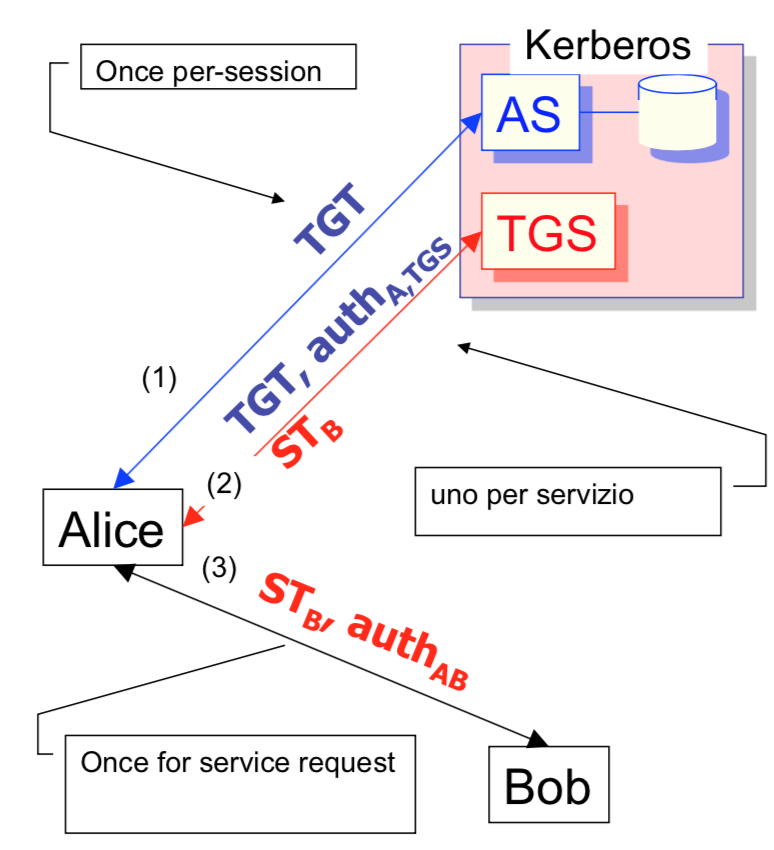
\includegraphics[width=0.3\textwidth]{img/tgs}
\end{figure}

At login, A receives the \textit{Ticket Granting Ticket} (TGT) from AS in order to talk with the TGS to which A asks for \textit{Service Ticket} (ST), needed to talk with the system servers.

\subsection{Delegation problem}
\begin{figure}[H]
  \centering
  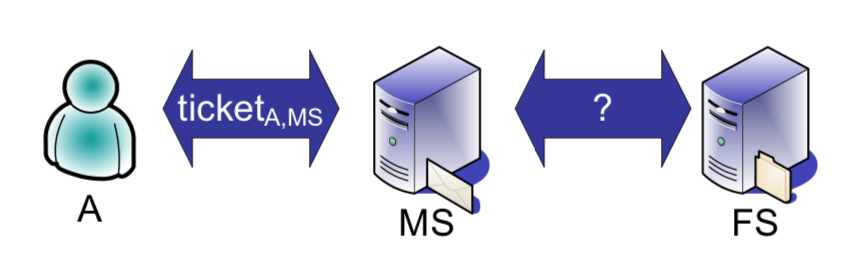
\includegraphics[width=0.4\textwidth]{img/delegation}
\end{figure}

Let assume that a mail server MS has to store A's mails in the file server FS: MS has to operate on behalf of A.

\subsubsection{Proxy tickets}

\begin{figure}[H]
  \centering
  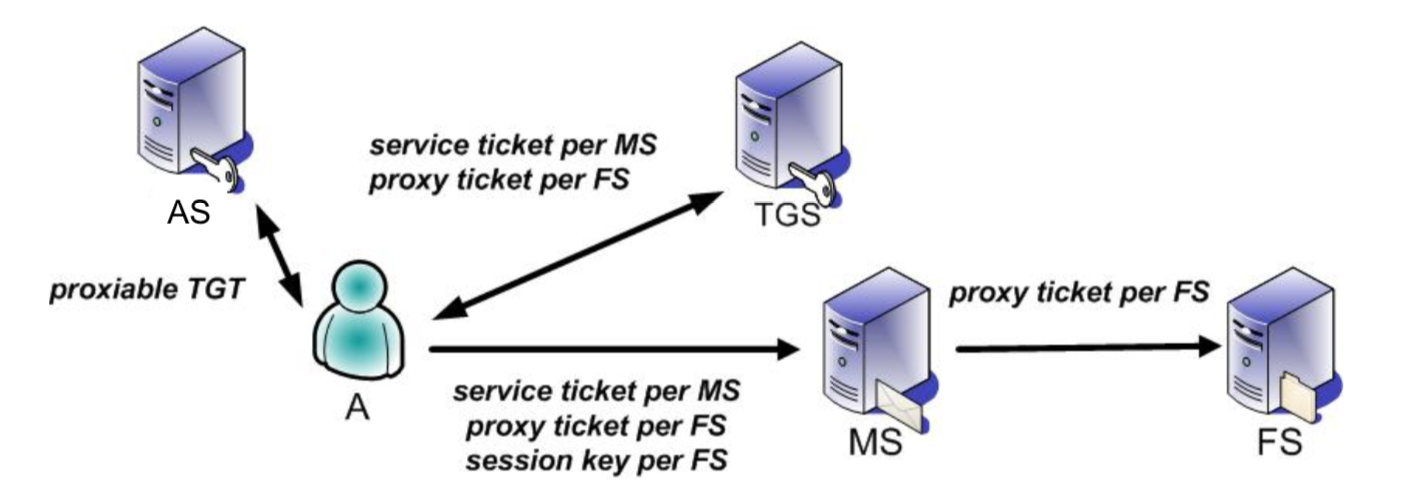
\includegraphics[width=0.5\textwidth]{img/proxy}
\end{figure}

Proxiable TGT allows A to ask the TGS a service ticket $ST_{MS}$ and a proxiable ticket $PT_{FS}$.

MS could make damage only to FS and for limited specified in the $PT$. However A has to know the number of tickets needed by MS to make it fullfill the service correctly.

\subsubsection{Forwardable TGT}

\begin{figure}[H]
  \centering
  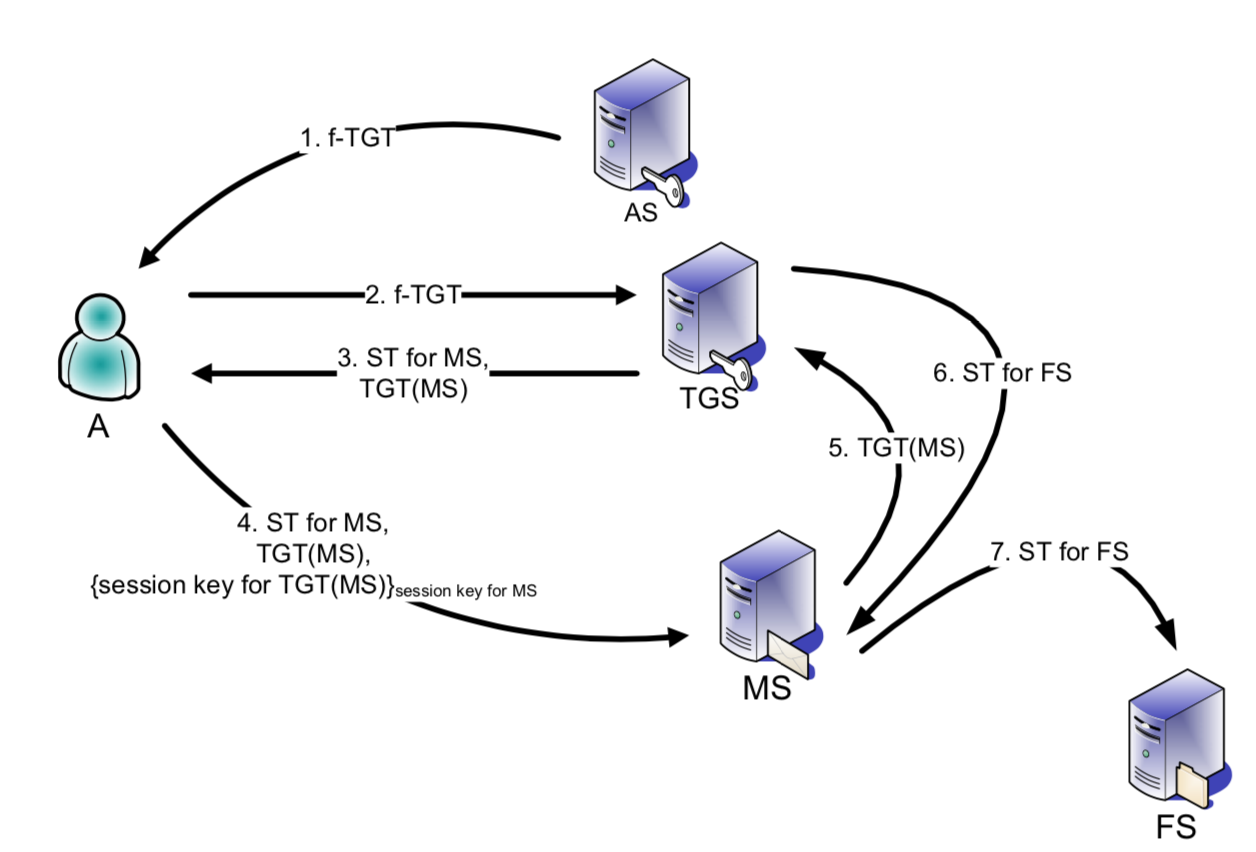
\includegraphics[width=0.5\textwidth]{img/forward}
\end{figure}

Forwardable TGT allows A to ask the TGS a TGT for MS. MS will use this TGT to ask TGS any $ST$ it needs.

A has not to know in advance the number of tickets for MS, but if MS gets compromised it can abuse of it.

\subsubsection{Referral TGT}

\begin{figure}[H]
  \centering
  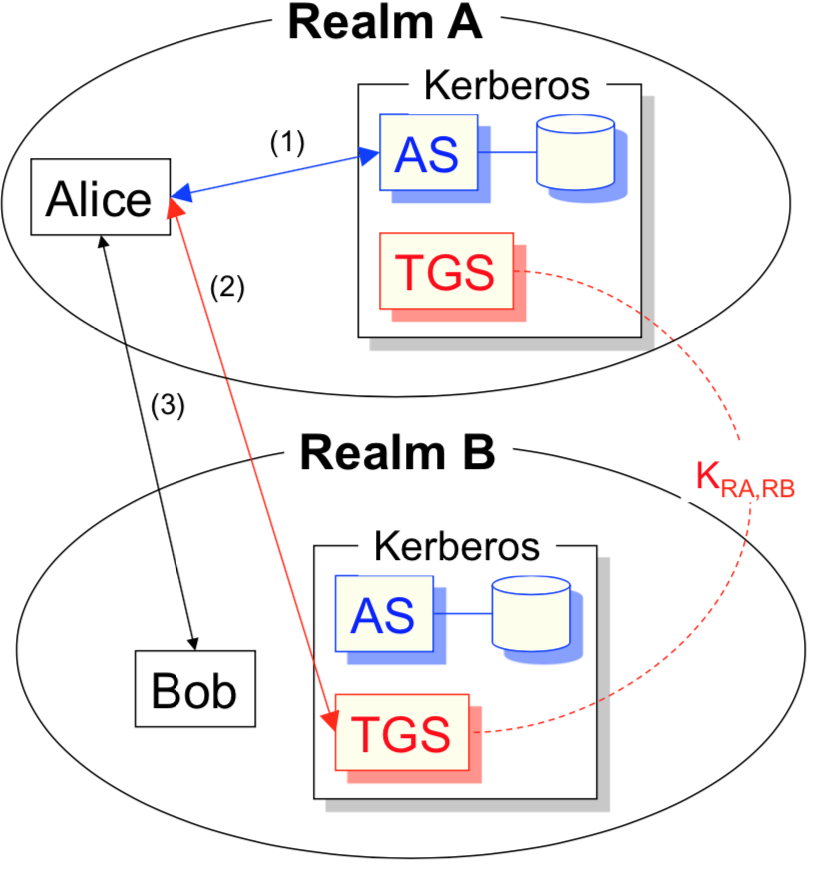
\includegraphics[width=0.3\textwidth]{img/realms}
\end{figure}
Referral TGT allows A to ask to a TGS of another \textit{realm} a $ST$ to interact with a server of that realm.

\newpage

\appendix

\section{Buffer overflow}
The data that overflows the buffer is written in the memory space that happens to be contiguous to the overflowed buffer, containing other data (variables, etc.). Therefore, other data is over-written.

The C and C++ languages are particularly susceptible to bugs leading to buffer overflow vulnerabilities. This is because they do not enforce implicit bounds checking on arrays, and they provide standard library functions (e.g., \texttt{gets()}) which do not enforce bounds checking. Moreover, they implement strings as null-terminated arrays of characters. This makes programming in C/C++ more error-prone than in other languages, for example the Pascal language which implements strings as couples $<$length, characters$>$.

A non-static variable in C/C++ can be allocated either dynamically (with \texttt{malloc()} or \texttt{new}/\texttt{new[]} operators) or automatically (by declaring it as a local variable in a function). The \textit{heap} is a memory space that contains all the dynamic variables, while the \textit{stack} is a memory space that contains all the automatic variables and the return addresses of the subroutines. A buffer overflow in the heap is called \textit{heap overflow}, while a buffer overflow in the stack is called \textit{stack overflow}. Both heap and stack overflows can read/change the value of other variables. Stack overflow is generally more dangerous, because it can directly change the execution sequence by changing the return address of the subroutines.

Different types of attack can be performed exploting buffer overoflow:
\begin{itemize}
	\item \textit{Arc injeciton}: the attacker makes the overflowed part corresponding to a valid address such that when the function returns, the execution flow will jump to the wanted instruction;
	\item \textit{Code injection}: the attacker makes the return address pointing to the first memory location of the injected malware. To mount a code injection, the attacker must know the exact address of the stack, which is not always predictable. To overcome this, the attacker can prepend the malware with a large number of NOP instructions (\textit{NOP slide}). The overwritten return address needs only to jump in the middle of the NOP slide, so it can be approximated. Then, the control flow will drop down to the malware code.
\end{itemize}

\subsection{Countermeasures}
The most common stack overflow protections are \textit{Data Execution Prevention} (DEP), \textit{Address Space Layout Randomization} (ASLR), and \textit{Stack Canaries}. None of these protections is definitive, because they do not make the attack impossible, but only more technically challenging.

\subsubsection{Data Execution Prevention}
DEP works by marking each part of the memory as executable or non-executable. The stack is marked as non-executable, so when the victim process tries to execute the malware in the stack, a fault is raised and the process abnormally terminates. Hardware-based DEP has a negligible impact on performance. Note that DEP prevents code injection, but it does not prevent arc injection.

DEP can be cheated with \textit{Return-Oriented Programming} (ROP) techniques. In ROP, malware is not injected but «built» with a sequence of victim code fragments, each of which ends with a return instruction (gadgets). The attacker injects the addresses of such gadgets in the stack. At the end of every gadget, the return instruction will make the instruction pointer jump to the next gadget. All the gadgets are located in executable memory, thus DEP is bypassed and the victim process does not abnormally terminate.

Depending on the victim code, it could not be possible to build complex malware (e.g., a shellcode) with gadgets. A simpler technique is to use the gadgets to build an API call that disables DEP on the victim process, which is much simpler. After that, the attacker can mount a «classic» code injection, by placing after all the gadgets’ addresses an additional address pointing to a location of the stack containing a complex malware.

\subsubsection{Address Space Layout Randomization}
In old operating systems, when a program was executed, it was always loaded in memory starting from address 0. This makes ROP easy, since the adversary knows deterministically all the addresses of the victim code. With \textit{Address Space Layout Randomization} (ASLR), the operating system decides randomically where to load the program to be executed. All the absolute addresses of the program code are relocated by the same random offset. Since the attacker does not know the relocation address, he cannot perform ROP because he cannot build the sequence of gadget addresses.

ASLR is an additional source of uncertainty for the attacker. However, it does not make the attack impossible, rather probabilistic. Indeed, the possible relocation addresses are few in the typical operating system. For example, Windows has only 254 possible random relocation addresses. The attacker could simply try several times to attack the process, until he guesses the correct relocation address. Moreover, the attacker can leverage \textit{pointer leaks}, that are program bugs that expose the value of pointers. If such pointers point to the code (e.g., a function pointer or the return address of a function call), they reveal the relocation address. Finally, the attacker could do ROP with gadgets from non-randomized memory, for example memory that contains the code of libraries shared between different processes.

\subsubsection{Stack canaries}
In the stack canaries technique, the prologue of every function pushes a value (canary) in the stack between the local variables and the return address. If an attacker wants to overwrite the return address with a buffer overflow, then he must corrupt also the canary. The function epilogue checks if the canary still has the correct value, and it raises an error if it has not.

The canary value must be unpredictable by the attacker. Usually, it is chosen at random at program execution, and stored in the thread-local storage. Stack canaries are a compiler-based protection technique.

Stack canaries are currently the most effective defense against stack overflow, because they are hard to bypass or to guess. Stack canaries are typically 4-byte long, so the attacker has a chance over $2^{32}$ to guess it. Stack canaries slightly slow down the program performance since they introduce some operations at the prologue and at the epilogue of every function. Some compilers optimize the program by avoiding stack canaries in those function that they consider «safe» from stack overflow vulnerabilities. For example, a compiler could consider safe a function which does not declare local arrays, or declares small local arrays.
Although stack canaries are quite effective and efficient, note however that they can defend only against arc injection and code injection. They cannot defend against those types of stack overflows that do not overwrite the return address. For example, an attacker can use a stack overflow to overwrite variables that are stored in locations contiguous to the overflowed buffer. In this way, the attacker can cause an unexpected behavior of the program without corrupting the return address and the canary. In addition, it is still possible to use a stack overflow to simply produce an abnormal program termination, thus causing a denial of service. Moreover, stack canaries cannot prevent \textit{buffer over-reads}, that is overrunning a buffer’s boundary in a read operation. A buffer over-read can lead to information leaks. Notably, a buffer over-read in the stack can also leak the value of the stack canary, which could then be used to mount successive stack overflow attacks.

\newpage

\section{Secure coding}
\textit{Secure coding} studies those programming errors which have caused the most common, dangerous, and disruptive software vulnerabilities in the past, the remediation best practices and the \textit{risk assessment}, i.e., the probability that these errors are exploitable, the possible impact, and the remediation cost. Secure coding aims at protecting customers from money loss due to security incidents, and limiting the patch releases of software.

Secure coding is strongly language-dependent. As a general rule, the lower the programming language level is, the more error prone, and thus the more susceptible to vulnerabilities. C and C++ languages are particularly error-prone, because they are intended to be lightweight and to produce a small codeprint. The programmer, especially if coming from higher-level languages like Java, may assume that the C language implicitly perform checks when it does not. Moreover, C and C++ follow the \textit{power-to-the-programmer} philosophy, that they do not prevent the programmer from doing what needs to be done. So they always consider the programmer to be fully aware of the consequences of the code he is writing. Despite their poor security characteristics, C and C++ are widely used still today, in particular when performances are a requirement (e.g., constrained/embedded devices or high-load servers) and when legacy code must be maintained.

\subsection{Undefined behavior}
An \textit{undefined behavior} is a behavior on which the C/C++ standard poses no requirements, for example in case of out-of-bound buffer access, null pointer dereferencing, or signed integer overflow. An \textit{unspecified behavior} is a behavior on which the C/C++ standard gives two or more possibilities, for example the order of argument evaluation in a function call. An \textit{unexpected behavior} is a well-defined behavior, yet unexpected by the programmer, due to incorrect programming assumptions. The majority of software vulnerabilities is based on undefined behaviors. The attacker tries to induce the program to perform undefined behaviors by means of special crafted inputs. Then, the attacker tries to damage somehow the system. Undefined behaviors must be avoided. Unspecified behavior must be known. Unexpected behaviors must be expected.

\subsection{Taint analysis}
Data that comes from a source external to the program (network, user input, file, command line arguments, environment variables, other software, etc.) and that has not been sanitized yet is called \textit{tainted data}. The result of an operation over tainted data is tainted data too. An operand or a function argument whose domain (i.e., the set of valid values) is a subset of the domain of its type (i.e., the set of all the possible values) is called \textit{restricted sink}. Undefined, unspecified and unexpected behaviors happen when tainted data is given as input to a restricted sink.

\subsection{Sanitization}
\textit{Sanitization} is an operation that removes the taint from a data. Sanitization can be done by \textit{replacement} or \textit{termination}. Replacement replaces out-of-domain values with in-domain values, while termination terminates the execution path of the entire program or the current operation.

\subsection{Strings}
In C, there is not a native string type. Strings are implemented by arrays of characters, with a special character (\textit{string terminator}) to indicate the end of the string. The array capacity must always be greater or equal than the string length + 1, to accomodate the terminator at the end. No terminator character is allowed inside the string.
The absence of a native string type and the intrinsic insecurity of the C string library functions can lead to many vulnerabilities, some of which are hard to correct. The C++ standard introduces the \texttt{std::string} type which is far less error-prone.

\begin{center}
\begin{tabular}{|l|l|l|}
\hline
Vulnerable & C countermeasure & C++ countermeasure \\
\hline
\texttt{gets(buf)} & \texttt{fgets(buf,size)}/\texttt{gets\_s(buf,size)} & \texttt{getline(cin,buf)} \\
\hline
\texttt{scanf(buf)} & \texttt{scanf("\%1023s", buf)} & \texttt{cin >> buf} \\
\hline
\texttt{sprintf(dest,"\%s",src)} & \texttt{sprintf(dest,"\%1023s",src)} & \texttt{dest=(string)src} \\
\hline
\texttt{strcpy(dest,src)} & \texttt{strcpy(dest,src,size)} + terminator & - \\
\hline
\end{tabular}
\end{center}

\subsection{Pointer subterfuge}
The attacker is able to perform an arc injection by overwriting the \texttt{func\_ptr} variable to point to a different function than \texttt{good\_func()}. This attack is an example of pointer subterfuge. A pointer subterfuge is the act of maliciously change a pointer to an object or a function before the victim program uses it.

A C/C++ program implicitly uses many function pointers, some of which are susceptible to pointer subterfuge. An example is the \textit{Global Offset Table} (GOT) in Linux, which contains pointers to global objects and functions whose addresses are unknown at compile time. The GOT contains the addresses of dynamic library functions like strcpy(), printf(), exit(), etc. The address of the GOT is fixed at compile time and it is not relocated at execution time. Moreover, the GOT resides in a writable part of memory.

\subsection{Dynamic memory management}
In C, the \texttt{malloc()} function must always be checked for allocation failure. C++ is safely than C regarding memory allocation/deallocation. Indeed, the \texttt{new} and \texttt{new[]} operators (by default) raise an exception if the allocation fails, so it is harder to forget to handle such error than using \texttt{malloc()}.

However, STL containers like \texttt{std::vector} and STL iterators are not much safer than “classic” C arrays, since they follow the same power-to-the-programmer philosophy, and they are efficiency-oriented. Indeed, using \texttt{std::vector} with functions that do not check for bounds (i.e. \texttt{std::copy()}) does not prevent from out-of-bound accesses.

A possible solution is to use \texttt{vector.at()} for accessing a \texttt{vector} element.

\subsection{Vector iterators}
C++ iterators are very powerful and they permit the programmer to do things impossible with higher-language iterators, for example with Java iterators. One of these things is the on-the-fly modification of containers.

\begin{lstlisting}[language=C++, basicstyle=\ttfamily]
void func(std::vector<int>& c){
	for(auto i = c.begin(); i != c.end(); i++){
		c.insert(i, val); // -> i = c.insert(i, val)
		i++;
	}
}
\end{lstlisting}

The \texttt{insert()} method could cause the reallocation of the \texttt{std::vector} internal buffer in case its capacity was not enough to accomodate the new element. In such a case, all the old iterators will be invalidated. The subsequent dereferencing of an invalid iterator constitutes an undefined behavior (typically, a read or write in unallocated memory).

In general, all the methods that invalidate iterators (e.g., \texttt{insert()}, \texttt{erase()}, \texttt{push\_back()}, \texttt{pop\_back()}, etc.) must be used carefully inside iterator-based cycles. The STL standard specifies which method of which container may invalidate which iterator. The standard solution is to use the return value of the \texttt{insert()} method, which always returns a valid iterator pointing to the newly inserted element. The \texttt{erase()} method return a valid iterator pointing to the element successive to the erased one.

\subsection{OS command injection}
The program uses \texttt{system()} function for executing shell commands, for instance sending email to an address specified by the user. An attacker could pass an address concatenated to a malicious shell command. The \texttt{system()} function is an interface to a command interpreter (the shell), which could receive as input special characters resulting in the execution of commands unexpected by the programmer. In general, strings passed to command interpreters like the shell, external programs, SQL interpreters, XML/Xpath interpreters, etc. should be sanitized before.


Sanitization can be performed with a character \textit{white list} (list of only-allowed characters) or character \textit{black list} (list of disallowed characters). Whitelisting is always recommended, because it is easier to identify “safe” characters than identify “unsafe” ones. If a white list is incomplete, this only constitutes a missing functionality (and not a vulnerability), which can be easily detected. Conversely, if a black list is incomplete, this constitutes a vulnerability, which can be hardly detected.

The call of \texttt{system()} is problematic and the CERT secure coding standard always discourages it. Process forking and calling \texttt{execve()} or \texttt{execl()} are recommended instead. In addition to unsanitized tainted strings, \texttt{system()} is dangerous if:
\begin{itemize}
	\item A command is specified without a path, and the PATH environment variable is changeable by an attacker. (The PATH variable specifies the default paths where the command processor finds executables to launch);
	\item A command is specified with a relative path and the current directory is changeable by an attacker;
	\item The specified executable program can be replaced (spoofed) by an attacker.
\end{itemize}

\subsection{TOCTOU race condition}
A \textit{time-of-check/time-of-use} (TOCTOU) race condition occurs when two concurrent processes operates on a shared resource (e.g., a file), and one process first accesses the resource to check some attribute, and then accesses the resource to use it. The vulnerability comes from the fact that the resource may change from the time it is checked (time of check) to the time it is used (time of use). In other words, the check and the use are not a single atomic operation. The shared resource can be a hardware device, a file, or even a variable in memory in case of a multi-threaded program.
This program writes a given file only after having checked that the file does not exist, to avoid overwriting it. However, the time of check is different to the time of use, so a TOCTOU race condition is possible. Assume that an attacker wants to destroy the content of a file over which she has not write permission. Assume further that the TOCTOU-vulnerable program runs with higher privileges. To induce the program to overwrite the file content, the attacker can create a symbolic link to the file just after the time of check but just before the time of use.

To avoid the TOCTOU race in this case, it is sufficient to use the "x" flag when opening the file (since C11), which forces the \texttt{fopen()} function to fail in case the file already exists.

TOCTOU race conditions are typically easy to identify, but not always easy to correct in general. Sometimes it is better to mitigate the vulnerability in other ways, rather than avoiding the TOCTOU race itself. For example, we can simply run the program as a non-privileged user, or we can read/write files only in «secure directories», i.e., directories in which only the user (and the administrator) can create, rename, delete, or manipulate files.

\subsection{Integers}
The C standard imposes the unsigned integers to be represented with their binary representation, while allows the signed integers to be represented with three techniques: sign-and-magnitude, one’s complement, two’s complement. The most used representation in desktop systems is however two’s complement.

The majority of platforms use two’s complement representation, and silently wrap in case of signed integer overflow. Many programmers rely on this usual behavior as if it were the standard one, but it is not. Notably, compilers leverage the assumption that no integer overflow happens in order to implement code optimization. So the actual behavior could vary on the compiler, the compiler version, and the single piece of code.
Despite the fact that the integers are used primarly for sizing and indexing arrays, for which the presence of the sign is meaningless, the signed integers are traditionally the most used integer types in C and in many modern programming languages.

\subsubsection{Unsigned sanitization}
A general method to sanitize integers before potentially overflowing operations is the following:
\begin{enumerate}
	\item Identify how an arithmetic operation could overflow, and write the error condition «as is», i.e., as if no overflow would happen within the error condition itself;
	\item Algebrically change the condition to avoid overflow inside the error condition itself;
	\item Possibly avoid the additional overflows in the error condition just obtained.
\end{enumerate}

\begin{center}
\begin{tabular}{|l|l|}
\hline
Sum & \texttt{a > UINT\_MAX - b} \\
\hline
Subtraction & \texttt{a < b} \\
\hline
Increment & \texttt{a == UINT\_MAX} \\
\hline
Decrement & \texttt{a == 0} \\
\hline
Multiplication & \texttt{b != 0 \&\& a > UINT\_MAX/b} \\
\hline
Division and modulo & \texttt{b == 0} \\
\hline
\end{tabular}
\end{center}

\subsubsection{Signed sanitization}
Sanitizing operations with signed integers is in general more difficult than unsigned integers. This is because signed operations typically can overflow in both directions: beyond INT\_MAX and below INT\_MIN. For example, a signed sum can overflow beyond INT\_MAX if the operands are both positive, or below INT\_MIN if they are both negative.
The simplest countermeasure is to sanitize the signed integers to be non-negative, thus making them unsigned. Then, apply the sanitization rules for the unsigned ints seen before. However, sanitizing away the negative values is not always possible, as they may be valid values of the program. Another solution is to tell the compiler to raise an exception on integer overflows, so that the program crashes instead of going in undefined behavior. GNU GCC compiler allows to do that with the \texttt{-ftrapv} flag. The \texttt{-ftrap} flag forces the integer overflow to raise an exception, which by default results in a program termination. This makes a program more secure, but also less efficient because it causes implicit function calls in every signed operation and prevents some hardware optimizations. Moreover, it does not cover all the signed operations, so it is a partial solution. Another solution is to apply the general sanitization method twice, once for each overflow direction.

\begin{center}
\begin{tabular}{|l|l|}
\hline
Sum & \makecell[l]{\texttt{b >= 0 \&\& a > INT\_MAX - b} \\ \texttt{b <= 0 \&\& a < INT\_MIN - b}} \\
\hline
Subtraction & \makecell[l]{\texttt{b <= 0 \&\& a > INT\_MAX + b} \\ \texttt{b >= 0 \&\& a < INT\_MIN + b}} \\
\hline
Increment & \texttt{a == INT\_MAX} \\
\hline
Decrement & \texttt{a == INT\_MIN} \\
\hline
Multiplication & \makecell[l]{\texttt{(b > 0 \&\& a > INT\_MAX/b)||(b < 0 \&\& a < INT\_MAX/b)} \\ \texttt{(b > 0 \&\& a < INT\_MIN/b)||(b < -1 \&\& a > INT\_MIN/b)}} \\
\hline
Division and modulo & \makecell[l]{\texttt{b = 0} \\ \texttt{b == -1 \&\& a == INT\_MIN}} \\
\hline
\end{tabular}
\end{center}

\newpage

\section{Network security}
\subsection{Penetration test}
A \textit{penetration test} (pen test, in brief) is an authorized simulated attack to a computer system. The aim is to determine the security level of a system and report to the system’s owner the possibly found vulnerabilities. A penetration test can be white-box, black-box, or gray-box. In \textit{white-box} penetration tests, the pentester is given full knowledge of the system details, and the organization is aware that a penetration test is ongoing. White-box pen tests are generally cheaper and quicker, and they can find lots of vulnerabilities. However, they are generally less realistic. In \textit{black-box} penetration test, the system details are hidden to the pentester, and (most of) the organization is unaware that a penetration test is ongoing. Black-box pen tests are more expensive, and they usually find only the easiest and most exploitable vulnerabilities. However, they are more realistic, and they also evaluate the reaction capabilities of the security team of the organization. \textit{Gray-box} pen test are a mix of white-box and black-box.

\subsection{Exploitation}
An \textit{exploit} is a piece of software that takes advantage of a vulnerability to cause some damage on a computer. Such damage includes executing arbitrary code, escalating privileges, or performing a denial-of-service attack. If the exploit aim at executing code, the malware being executed is called the \textit{payload} of the exploit. Examples of payloads are remote shells, spam-sending programs, self-replicating worms, etc. An \textit{exploit kit} is a collection of exploits and payloads. A famous and widespread exploit kit is Metasploit framework.

\subsection{Network scanning}
\textit{Network scanning} is a collection of techniques aimed at discovering hosts and services on a network by sending packets and analyzing the responses. An example of network scanner is \textit{nmap}.
Network scanning usually involve \textit{host discovery}, that is enumerating particular hosts on a network, for example those responding to ICMP requests or having a given port open, and \textit{port scanning}, that is enumerating open/reachable ports on a given host.

\subsubsection{SYN scanning}
Port scanning is usually done by \textit{SYN scanning} (aka TCP half-open scanning), which consists in initiating a TCP connection establishment with a given host/port without completing it. The network scanner sends a SYN packet to the target port and observes the response. If the target responds with a SYN-ACK packet, then the port is open to accept connections. The network scanner can possibly abort the connection by sending a RST packet. If the target responds with a RST-ACK packet, then the port is closed and it does not accept incoming connections. If the target does not respond at all, then the port could be filtered by a firewall. SYN scanning has the advantage that it consumes few resources on the target host, because no TCP port is left open.

\subsubsection{UDP scanning}
Scanning UDP ports is more difficult because the protocol does not provide acknowledgement in case of open ports like TCP does. In particular, it is difficult to distinguish the open and the filtered state since many UDP applications will simply ignore unexpected packets. To perform UDP scanning, the network scanner sends a probe UDP packet to the target port, typically with an empty payload. If the target responds with an ICMP type 3 code 3 packet (port unreachable) or an ICMP type 3 code 13 (administratively prohibited) packet, then the UDP port is closed. If the target does not respond within a timeout, then the UDP port could be open as well as filtered by a firewall.

\subsubsection{Service scanning}
\textit{Service scanning} is a technique aimed at determining the type and the version of a server reachable at a given port. It works by sending one or more protocol-specific messages to the port, and analyzing the responses. For example, sending a \texttt{GET / HTTP/1.1} probe to the port 80 could detect a web server, and the response could give indications about which server and which version of such server. Note that service scanning in some cases can also discriminate between open and filtered UDP ports.

\subsection{TCP/IP stack fingerprint}
\textit{TCP/IP stack fingerprinting} (aka OS fingerprinting) is a technique aimed at determining the type and the version of the operating system running on a given host. It works by analyzing implementation-dependent TCP/IP parameters. Some parameters of the TCP protocol are not strictly defined by the specifications, and they are left up to the implementation. Different operating systems, and different versions of the same operating system, set different default values for these parameters. By analyzing these values, the network scanner can distinguish the type and the version of the operating systems and of the TCP/IP stack implementations. A typical parameter used for fingerprinting is the initial Time-To-Live (TTL) of the IP packets, which is usually small for older operating systems and large for newer ones. This reflects the fact that the number of hops of the average TCP connection increases as the years go by, due to the increasing complexity of the Internet. Since the TTL of an IP packet gets decremented at each hop, the network scanner must know the number of hops from the target to infer the exact initial TTL. Another typical parameter is the TCP window size, which tells how much data the receiver can accept before acknowledging the sender.

\subsection{Network sniffing}
\textit{Network sniffing} (aka passive network scanning) is a technique aimed at eavesdropping and analyzing traffic in a local area network, in order to steal unencrypted data or gain information like available hosts, open ports, available services, etc. An example of network sniffer is wireshark. Network sniffing can gain the same information that network scanning can, including service type/version and operating system type/version, but in a completely stealthy way. It requires the attacker to be in the same local area network of the target hosts.

\subsection{Fuzzing}
\textit{Fuzzing} (aka fuzz testing) is a testing technique that automatically provides to a target software a long series of invalid, unexpected, or totally random inputs with the aim of finding implementation bugs and vulnerabilities. Examples of inputs are network messages, but also keyboard and mouse events or files. The attacker monitors the target software for faults. If the attacker can execute the target software locally, she can monitor also for unexpected internal states and memory leaks. Common examples of fuzzers are \textit{American fuzzy lop} and \textit{Peach fuzzer}.

\textit{Generation-based} fuzzing produces (semi-)random inputs from scratch. On the contrary, \textit{mutation-based} fuzzing produces inputs by randomly modifying some seed input configured by the tester. \textit{Dumb} fuzzing produces completely random inputs, without knowing the input structure. On the contrary, \textit{smart} fuzzing produces inputs basing on a formal model of the input structure.

\newpage

\section{Malware}
In the past ('80-'90), the virus writers were principally young male programmers wanting to prove their skills to the community of “black hats”. Nowadays, malware is developed mainly for business, politic, or espionage purposes. Political activists typically write malware to attack a specific website of a company or organization. Criminals develop malware in order to show paid-per-click advertisements, or to steal and sell passwords, credit card numbers, or personal information. Moreover, they can blackmail victims by blocking their computer and demanding a ransom to unblock them, or they can simply sell malware to other parties (black market). Finally, intelligence agencies develop malware to steal strategic information from world leaders, or to perform industrial espionage or industrial sabotage.

Modern malware is hard to classify rigidly, because it usually has different features. An important classification is based on its infection paradigm (if any): 

\begin{itemize}
	\item \textit{Virus} is a piece of code that infects a file, typically executables or any files capable of containing code (e.g., .doc, .pdf, etc.), and it self-replicates to other files. Actually, viruses are rare nowadays, because their infection is easy to detect by anti-virus software. However, the term “virus” is also used to indicate a generic self-replicating malware;
	\item \textit{Worm} is a program that infects a computer (not a single file, like viruses do), and it self-replicates to other computers through a network. Worms are the most common kind of self-replicating malware nowadays;
	\item \textit{Trojan horse} (or Trojan) is a malicious program that appears to be legitimate, thus misleading the user about its true intent. It usually does not self-replicate, and it infects the victims by social engineering (e.g., an hacker that sends an email with malicious attachment);
	\item \textit{Spyware} collects information about the user;
	\item \textit{Keylogger} records the key strokes to steal passwords;
	\item \textit{Adware} shows advertising to the user, and it is not necessarily malware. It is considered malware if the user did not give his consent to receive such advertising;
	\item \textit{Rootkit} grants privileged access to the host system;
	\item \textit{Dialer} performs phone calls to premium numbers;
	\item \textit{Botnet} is a network of infected computers receiving orders from a Command and Control point (C\&C). It is typically used to launch Distributed Denial of Service (DDoS) attacks against a specific target;
	\item \textit{Ransomware} typically encrypts user information and then asks the user a ransom in bitcoins or other cryptocurrencies for the decryption key;
	\item \textit{Scareware} displays messages to cause panic and anxiety in order to lead users into buying other software. Most scareware presents itself as security software, and it deceives users into believing their computer is infected by a virus;
	\item \textit{Cryptominer} uses victim's computer to mine cryptocurrencies.
\end{itemize}

\subsection{Common features}
The only feature common to all malware is \textit{infection}, that is, the capability of executing the first time on a host against the will of the user. To do this, malware can leverage poor precautions by the user and/or security vulnerability of some software components. An infection technique is also called \textit{infection vector}. Malware can be \textit{persistent}, which means that it keeps the host infected after a reboot. Malware can \textit{self-replicate}, that is, it can automatically infect other hosts with copies of itself. Malware can adopt \textit{concealment} techniques, in order to avoid being detected by the user or by anti-virus software. Malware can perform \textit{privilege escalation}, that is gain higher privileges on the host machine in order to bypass access control mechanisms. Finally, malware can \textit{damage} the host and/or other victims.

\subsubsection{Infection and self-replication}
There are countless infection and self-replication mechanisms. The most common ones involve social engineering, for example sending emails with Trojan attachments, or deceiving users into downloading infected files from malicious (or poorly controlled) websites. The file names with a double extension (e.g., “.jpg.exe”) leverage the default behavior of Windows systems which hide the real extension “.exe” to the user. The user thus sees the file as having an innocuous file extension (e.g., “.jpg”). Another common infection method is to bruteforce authentication with a database of default or commonly used username/password couples (e.g., admin/admin).

A lot of malware also infects mounted removable drives (e.g., USB memory sticks) and copies itself on them in autorun configuration. Another common method is sending malformed messages to vulnerable processes, in order to leverage bugs (e.g., buffer overflows) that allow arbitrary code execution on the victim machine.

\subsubsection{Persistency}
\textit{Persistency} is the ability of self-execute after reboots. Viruses typically prepend themselves at the beginning of legitimate executable files. Worms can leverage many persistency techniques, for example register themselves as start-up programs. In Windows systems this can be done by writing certain keys in the system registry.

Another common persistency technique is \textit{DLL hijacking}, in which malware replaces a dynamic library (DLL in Windows, SO in Unix) with malware code. Every time a legitimate process calls some API function of the library, malware is executed. The malware code, after performing some malicious action, calls in turn the legitimate API function of the legitimate dynamic library, in order to conceal its presence.

Another method is to replace a legitimate interrupt handler with malware code (\textit{handler hijacking}). Every time a legitimate process triggers such an interrupt, malware is executed.

\subsubsection{Concealment}
\textit{Concealment} means hiding malware’s presence to the user and to the anti-virus software. In order to hide its presence to the user, malware usually chooses non-explicative or random process names, which go unnoticed among other legitimate process with non-explicative names. The same is done for malware installation files, if any.

Another concealment technique is \textit{process injection}. In this case, the malware injects its code inside another legitimate process and executes it. This is allowed in modern operating systems (Windows, Unix, etc.) mainly for debugging purposes. In this way, malware conceals from detection and accesses the resources of the injected process.
In Windows systems, process injection can be done by means of the \texttt{CreateRemoteThread()} API function, which creates a thread that runs in the address space of another process. This is also called \textit{DLL injection}, because it requires malware to reside in a .DLL file.

More complex techniques are possible:
\begin{enumerate}
	\item An application (or the user) wants to view the list of the active processes;
	\item In the process list, among legitimate processes, there is the worm's process. The malware wants to hide it;
	\item The malware hijacks the library call that retrieves the active process list. It intercepts the system call and cancels its name from the actual list;
	\item The application (or the user) views the “clean” list.
\end{enumerate}

\subsubsection{Damage}
Malware can damage the host system or perform unwanted actions. The type and nature of these actions reflects the original intent of the malware writers. If the intent is to prove hacking skills, malware only displays funny messages or does some random damage, for example it deletes random documents or images or audio/video files. If the intent is to do activism, malware can remain silent for long times and then, upon receiving a specific message from a command and control point, it can send lots of requests to some target web site to realize a distributed denial of service (DDoS) attack. This behavior is typical of botnets.

If the intent is to earn money, malware can display unwanted paid-to-click advertisement (adware), or use victim’s processing power to mine cryptocurrency (cryptominer), or leak personal data which can be sold afterwards (spyware). Malware can encrypt victim’s documents and ask a ransom for decrypting them (ransomware). A typical ransomware dowloads a public key from a command and control point, and then it encrypts document files with such a key. Finally, it reveals itself by displaying a message to the victim with the instructions to pay the ransom. The victim cannot decrypt the files without the corresponding private key, which is owned by the command and control point. The ransom must be paid with an anonymous method, typically a cryptocurrency transfer. After the ransom is paid, the attacker gives to the victim a decryption program which embeds the private key.

If the writer’s intent is investigation or espionage, malware can record the victim’s actions in multiple ways: by microphone, camera, key strokes, browser history, etc.

\subsection{Anti-Virus software}
The main functionalities of anti-virus software are: 
\begin{enumerate}
	\item Prevent malware's infection;
	\item Detect malware's infection;
	\item Remove malware's infection.
\end{enumerate}
The first two features require the ability to recognize malware from legitimate software. Modern anti-virus software has other features, among which firewall, intrusion detection, anti-spam, and anti-phishing.

\subsubsection{Fred Cohen's result}
Fred Cohen (the inventor of the word “computer virus”) developed the following theorem:
\begin{center}
\textit{“A perfect malware detector is impossible”}
\end{center}
A proof by contradiction follows:
\begin{enumerate}
	\item Let us suppose a function \texttt{is\_malware()} exists, which examines a piece of code and returns true whether such a code is malware, false otherwise. Let us suppose that \texttt{is\_malware()} is perfect, that is it does not give any false negatives nor false positives. 
	\item Then, it is possible to build a program named \texttt{my\_program()}, which executes \texttt{is\_malware()} on itself. It behaves like a malware if the function return false, it does nothing otherwise.
	\item \texttt{is\_malware(my\_prog)} cannot return neither true or false. If it returns true, then \texttt{my\_prog()} will not be malware, thus it will be a false positive. If it returns false, then \texttt{my\_prog()} will be a malware, thus it will be a false negative.
\end{enumerate}
Hence, such a perfect malware detector is not possible.

\subsubsection{Signature-based detection}
The real-life anti-virus software tries to recognize malware by means of two main techniques: \textit{signature-based} detection and \textit{anomaly-based} detection.
A signature is a sequence of instructions in the code of a piece of malware, which univocally identifies it. The presence of a signature reveals the presence of malware inside an infected file or a running process.

The signature-based detection relies on a database of malware's signatures. Every suspect file and process are checked to contain such signatures. Signature database must be periodically updated by anti-virus software.
Such a method is efficient, gives very rare false positives, and identifies the specific piece of malware, rather than detecting its presence only. The identification is particularly important for the sake of removing it, as different malware requires different removal procedures. This is the most used detection method by anti-virus software.
The main drawback is that this method cannot recognize new malware, whose signature has not been isolated yet. Another drawback is that it does not protect against polymorphic malware, as we will see in the following.

Malware can self-encrypt itself in order to avoid signature-based detection. The decryptor and key are stored in the clear before the encrypted malware's code. During the first execution, the decryptor recovers malware's code and executes it. During the self-replication phase, the malware chooses a new random key and encrypts its code.
Note that a strong encrypting algorithm is not needed here. The encryption aims only at avoid the detection, rather than protecting the confidentiality. Very simple encryption algorithms like XOR masks are often used.

This concealment technique is easy and efficient, but malware can still be recognized by means of the decryptor code. Such a code does not vary between infections, thus it can be used as a signature. However, self-encryption is still useful to avoid detection since it significantly reduces the code where the signature can be found.

A more advanced technique is \textit{polymorphism}, which consists in changing the malware code without changing its behavior. A simple polymorphism technique is inserting NOPs (NO Operation) at random locations inside code. Another technique is to insert ineffective operations, like increments and successive decrements of the same registers. A third technique is to reassign registers, for example replace EBX to EAX.

\subsubsection{Sandbox-based detection}
Sandbox-based detection tries to detect malware by executing suspect software inside \textit{sandboxes}, which emulate real hardware in a controlled and isolated manner. Malware must be unaware to be running inside a sandbox. All the actions of the suspect software are logged, and then the logs are analyzed to detect malware behavioral fingerprints. This detection technique can protect against self-encrypting malware, polymorphic malware, and variants of known malware. However it is slower and less efficient, so it is rarely used in end-user antivirus software.

Moreover, malware can prevent being run inside a sandbox, or detect it at runtime by accessing non-emulated resources. For example, it can use instructions performed by the Floating Point Unit (FPU). Specific tools exist which replace normal operations with FPU operations. If malware detects to be running inside a sandbox, it typically stops all malicious operations.

\subsection{Reverse engineering}
Reverse engineering is the process of analyzing a software system in order to create a higher-level representation of it. Reverse engineering can have many purposes, among which malware analysis.
A simple reverse engineering technique is text extraction, which aims at recoverying sequences of printable characters from the executable code. It can extract output messages giving hints on the program’s functionalities, or sensitive information like hardcoded passwords. If the executable code includes debug metadata, text extraction can also extract the names of the functions declared in the program and in statically-linked libraries, which give further hints on the program’s functionalities. An example of text extractor is the “strings” command in Unix.

Library call tracing is another simple reverse engineering technique aimed at tracing all the calls that a program performs to dynamically-linked libraries (e.g., .DLL in Windows, .SO in Unix) with the relative parameter values. Library call tracing acts by inserting \textit{shims} between the target executable code and the shared libraries that it uses. A shim is a library that transparently intercepts calls. Library call tracing cannot trace calls to statically-linked libraries, because they are compiled in the same executable file of the program. An example of library call tracer is the \texttt{ltrace} command in Unix.

\subsubsection{Decompilation}
\textit{Decompilation} is a technique aimed at creating high-level language source code that (once re-compiled) behaves in the same way of a given executable piece of code. It is thus the inverse operation of compilation. Decompilation is one of the main techniques of reverse engineering, and it is extremely useful for analyzing malware and for cracking software protected by digital-rights management techniques. An example of decompiler is Ghidra.

Decompilation cannot usually reconstruct perfectly the original source code. The quality of the output source code mainly depends on the amount of information that can be extracted from the executable code. The presence of debug metadata helps decompilation since it makes it possible to reproduce the original names of the variables and the functions, as well as the line numbers. The bytecode-format executables used by Java or .NET virtual machines are usually easier to decompile since they contain a lot of metadata and high-level features.

Decompilation is a complex process composed by several phases: 
\begin{itemize}
	\item \textit{loading phase} involves the parsing of the input executable and the extraction of some information like the target architecture (Pentium, ARM, PowerPC, etc.), the employed compiler (gcc, Visual Studio, etc.), and the entry point of the program (i.e., the “main()” function);
	\item \textit{disassembly phase} translates the architecture-specific binary instructions into an architecture-independent representation called \textit{intermediate representation};
	\item \textit{program analysis} recognizes the high-level expressions (a=b*c, etc.);
	\item \textit{data flow analysis} recognizes the variables;
	\item \textit{type analysis} recognizes the variable types;
	\item \textit{structure analysis} recognizes the control-flow instructions (if, while, switch, etc.).
\end{itemize}

These phases work by isolating and recognizing idiomatic code sequences, that are sequences of instructions that a given compiler uses to translate high-level instructions.

\subsubsection{Obfuscation}
\textit{Obfuscation} is a technique aimed at producing executable code which is harder to reverse engineer. This can be done by removing metadata from executable code, and by compiling in such a way to hide idiomatic code sequences.

\newpage

\section{Web security}
The main technology behind any web application is HTTP (HyperText Transfer Protocol). HTTP uses a message-based model, in which a client sends an \textit{HTTP request} and the server sends back an \textit{HTTP response}. HTTP by itself is \textit{stateless}, in the sense that it does not require the server to maintain a state over multiple requests. However, web applications that are on top of HTTP maintain their state both at the server side (e.g., by means of \textit{session variables}) and at the client side (e.g., by means of \textit{cookies}).

The core security problem of web application (like all the types of applications) is that users can submit arbitrary input. However, in web applications this is particularly difficult to address, since the possible inputs are many. In practice, all the content of an HTTP request is tainted: the requested URL, the parameters, the HTTP headers, the request body, etc. In addition, requests can arrive in any sequence, thus we cannot assume a particular order in the page requests, for example the order given by the links in the HTML code. This is true also in a non-adversarial situation, because honest clients can press the back button, or bookmark URLs to access them directly, etc. Another assumption that we have to make is that attackers may not use (only) browsers to attack our web application. There are many tools available that permit attackers to change anything in the HTTP request, read anything in the HTTP response (for example cookies, hidden fields, and HTTP headers) and perform requests in quantity and rates impossible with normal browsers.

\subsection{Web application mapping}
There exist different actions for attacking web applications exploiting the HTTP protocol:

\begin{itemize}
	\item \textit{HTTP proxy} is a server that records, relays and possibly manipulates all the requests and the responses between a client browser and a web server. Attackers can use a local HTTP proxy when attacking web applications, in order to intercept and analyze HTTP requests and responses between her browser and the target application.
	\item \textit{Web spider} (aka web crawler) requests pages to a target web site, analyzes them to extract links to other pages, and then requests those pages recursively. Advanced spiders are able also to automatically fill up input forms, execute client-side scripts that possibly produce links. Web spiders are used for benign purposes (e.g., mapping a website for a web search engine) as well as for malicious ones. In the latter case, the aim is to completely map the web application in order to discover the functionalities and identify the most convenient attack surfaces. Of course, web spidering cannot discover hidden contents, such that pages that are not linked by the public pages of the website.

	The \textit{robots exclusion standard} is a standard method to inform spiders about which pages or areas of a website should not be spidered. It works by providing a “robots.txt” file at the root of the website hierarchy, which contains a blacklist of URLs that spiders should avoid. Of course, malicious spiders can ignore robots. Exclusion directives, or even start spidering exactly from those URLs, under the assumption that blacklisted URLs may contain the most sensible information or the most security-critical functionalities.
	\item \textit{Directory bruteforcing} is a technique that performs a large series of HTTP requests to a target website, trying different paths taken from a database of common directories, or combinations of them. The aim is to discover hidden content which is often security-critical, since it can contain hidden administrative functionalities or new features yet under alpha-testing. Hidden content can also contain backup copies of dynamic pages. If such copies have a changed file extension (e.g., “.php.bak”), then the web server could not identify them as executable. Thus, requesting these copies would enable the attacker to view the server-side source code, in order to find vulnerabilities. Moreover, hidden content can contain backup archives of dynamic pages, which can leak server-side source code as well.
\end{itemize}

\subsection{Authentication}
There is not a silver bullet to implement a secure authentication solution. Moreover, advanced security in authentication often means increased costs and decreased usability. The security criticality of the particular application must be considered when designing the authentication mechanism. More critical applications (e.g., e-banking) will need more security, less critical applications (e.g., a newsletter) will need more usability. The most secure solution is probably \textit{multifactor authentication}. In multifactor authentication, the user identity is confirmed on the basis of multiple pieces of evidence of different types, for example a password and a physical token. Typically, authentication factors are categorized in three types: what the user knows (e.g., a password), what the user has (e.g., a smart card or a physical token), what the user is (e.g., his/her fingerprints). However, multi-factor authentication is expensive and cannot be applied in every application.

\subsubsection{Strong credentials and password change}
The first and most effective countermeasure is to force users to choose strong credentials. Passwords should have a minimum length, they should be composed by lowercase, uppercase, numeric, and typographic characters, and they should avoid names and dictionary words. A password change functionality must be provided, in order to let users change their password in case they suspect it has been compromised.

\subsubsection{Secure credential transmission}
After having enforced the password quality, credentials must be protected from compromise. All client-server communications must be protected by well-established cryptographic protocols like HTTPS, especially the requests in which clients transmit their credentials. The web page presenting the login form must be transmitted by HTTPS too. Otherwise, users cannot verify the authenticity of the login page, thus it is not guaranteed that the credentials will be submitted to the real server.

Credentials should never be transmitted via URL parameters, for several reasons. First of all, URL parameters are displayed on screen on the URL bar of the browser, and this could lead easily to credential stealing. Moreover, if the user follows an off-site link leading to another website, the browser will include the old URL together with the parameters in the HTTP request, inside the “Referer” HTTP header. Finally, visited URLs are usually logged in several unsafe places, like browser’s history, server logs, and logs of possible proxy servers. Saving credentials in cookies is generally considered unsafe too, because they can be stolen via client-side attacks, for example cross-site scripting (see after). Se safest way to transmit credentials is inside the HTTP body (i.e., through a POST request), which is not displayed on screen, logged anywhere, or transmitted off-site.

\subsubsection{Secure credential storage}
Finally, credentials should be stored at server side in such a way that it is infeasible to recover the original value, even in case the server’s database gets compromised. A common way to do that is to store a salted (i.e., randomized) one-way hash function of the password. An example of hash algorithm for password storing is the \textit{BCrypt} algorithm, which is included in the PHP 5.5.0+ standard.

\subsubsection{Fail-Open Flaws}
The application logic that checks the credentials must be carefully designed to be free of fail-open flaws. A \textit{fail-open flaw} is a vulnerability in which an application grants access (instead of denying it) in case an error or exception is encountered. These kind of flaws are especially prevalent in those programming language strongly based on exception, for example Java. In these cases, a good practice is to surround the core authentication check with catch-all exception handlers which denies access.

\subsubsection{Verbose errore messages}
In case the user fails to login, the error message returned by the application should not give any hints (explicit nor implicit) about which part of the credentials is wrong, because this information could help attackers. For example, messages like “wrong password for user ‘Alice’” tells an attacker that a username “Alice” actually exists, thus leaving space for a user enumeration attack, which could allow the attacker to mount more \textit{dangerous attacks}. The application should always return the same generic uninformative message, for example “invalid credentials”.

\subsubsection{Account locking and CAPTCHAs}
Countermeasures must be taken to avoid bruteforcing against login mechanism, as well as against related mechanisms like password changing, password recovery, etc. Preventing user enumeration significantly mitigates the possibility of login bruteforcing. Another common mitigation is \textit{account locking}, which is a technique by which the authentication is suspended for a specific account for some time (e.g., 30 minutes) after a given number of failed login attempts (e.g., three). Account locking is considered safer than other similar locking countermeasures, for example session locking or IP address locking. With session locking, the application suspends the session after a given number of failed login attempts. However, an attacker can easily start a new session by deleting the session token. With IP address locking, the application suspends the client’s IP address after a given number of failed login attempts. However, an attacker can easily change her IP address.

In addition to account locking, another countermeasure against bruteforcing attacks are CAPTCHAs. A CAPTCHA (Completely Automated Public Turing Test to Tell Computers and Humans Apart) is a challenge-response test used to determine whether the user is human or not. A simple example of CAPTCHA is an image displaying distorted letters. The human user is able to reconstruct the original letters, and thus to solve the challenge. On the contrary, this is a hard problem for software, even if aided by machine-learning techniques.

\subsubsection{Account recovery}
User often forget their passwords. The account recovery functionality must be carefully designed to avoid possible vulnerabilities. The best way to implement an account recovery functionality is to send to the user an email (configured at registration time) carrying a unique, time-limited, unguessable, single-use recovery URL. When the user visits such an URL, (s)he is allowed to set the new password without exposing the old one in any way. To further protect the account recovery functionality, the application could present the user with a secondary challenge before sending the email, for example the name of his/her first school, and so on.

\subsection{Session management}
The security of a session management mechanism depends on how well a web application handle the related session tokens. Session tokens must be created in such a way they are unpredictable, and they should not have an internal structure nor meaning (even obfuscated). The best session tokens are long sequences of random bytes generated by a secure random number generator, and associated to server-side session data. All data about the current application state should be stored at the server side, and the session token should act only as a key to access it.

An alternative to random session tokens are encrypted session tokens. With encrypted session tokens, the current state of the application is entirely stored at the client side (e.g., with a cookie) in an encrypted form, typically by a symmetric key known only by the server. Although this technique makes the server more lightweight because it outsources all the state information to the clients, it is considered less secure and rarely used nowadays. Indeed, the security of all the web application depends on the strength of the encryption mechanism and on the symmetric key(s) used to encrypt and decrypt. If the encryption mechanism is somehow flawed, for example because it permits an attacker to forge or tamper with session tokens, or if the symmetric key(s) are not well-protected, then all the security is jeopardized. Moreover, this technique does not allow the server to perform data mining on the application states, which could be a valuable source of information.

\subsubsection{Secure token transmission}
After session tokens have been created, they must be protected from compromise during their entire lifecycle. Indeed, if an attacker steals somehow the token of an ongoing session of a legitimate user, she can inject requests on the same session, thus impersonating the user. This is called \textit{session hijacking attack}. First of all, tokens should be transmitted only over confidential channels, such as HTTPS. If HTTP cookies are used to transmit tokens, they should be flagged with the “secure” attribute. The “secure” attribute tells the browser that the cookie should be transmitted only over HTTPS. In this way, even if the website contains non-HTTPS pages (usually static resources like help pages) the session token does to risk being compromised.

Session tokens should not be transmitted in URLs, because this is unsafe for the same confidentiality reasons explained before for passwords: URLs appear on screen, on browser history, on server logs, etc. In addition to these reasons, sending session tokens in URLs exposes the users to session fixation attacks. In a \textit{session fixation attack} the attacker induces a legitimate user to follow a particular URL (e.g., by sending an email with a link inside) containing an untrusted session token, which has been previously created by the attacker herself. In this way, the attacker can obtain the same effects of a session hijacking.

\subsubsection{Session termination}
The application should implement a logout functionality, with which the users can delete all the server-side session information and invalidate the session token. However, users must not be supposed to explicitly log out at every session. Thus, sessions should also automatically expire after some inactivity period (e.g., 10 minutes).

\subsection{Code injection}
One of the most common and devastating attacks in the web is the \textit{SQL injection} attack. Bypassing authentication is not the only possible impact of a SQL injection. Other effects include escalating privileges, stealing data, adding or modifying data, partially or totally deleting a database.

The aforementioned problem is not specific of SQL, but of all the interpreted languages, for example LDAP, XPath, etc. Such languages are very prevalent in web applications, especially for interfacing back-end components like databases. In a typical web application, user-supplied data is received, manipulated, and then acted on possibly by means of some interpreter. In this case, the interpreter will process instructions of the web programmer mixed to user-supplied data. If this mix between instructions and tainted data is not done properly, an attacker can send crafted input that breaks out of the data context, usually by injecting some syntax that has a meaning in the interpreted language. As a result, part of the attacker’s input is interpreted as code (\textit{code injection}) and executed as legitimate code written by the programmer.

\subsubsection{Tautology}
The \textit{tautology} technique consists in injecting a condition wich always evaluates to true (e.g., 1=1) in a WHERE clause in order to bypass it somehow. Imagine the following SQL statement:

\begin{lstlisting}[language=SQL, basicstyle=\ttfamily]
SELECT * FROM users WHERE pwdHash='$pwdHash' AND name='$name'
\end{lstlisting}

In this case, the simple commenting technique cannot be applied. However, the attacker can bypass authentication anyway with the tautology technique, by injecting the following input: \texttt{\$name = admin' OR 'a'='a}.
Since the WHERE clause is always true, then the query will return all the tuples of the ‘users’ table. Thus the attacker can bypass the authentication. Note that here we did not use a trailing comment symbol (\texttt{--}) but a more «elegant» quote balancing technique, which consists in injecting an even number of quotation marks in such a way all string literals are «closed» in the resulting query, thus avoiding syntax errors. The final effect is the same as using the comment symbol, but quote balancing works even in the case the comment symbol is sanitized by the application.
The clause commenting and the tautology techniques can also be used to steal data. For example, a webpage that displays some information of the current user can be forced to display information of all the users by making the WHERE clause evaluate always to true.

Moreover they can be used not only with SELECT statements, but only with INSERT, UPDATE and DELETE statements.

\subsubsection{Finding SQLI bugs}
There is a “safe” test to find out (without damaging the database) whether a user-supplied input is injectable and it is incorporated into a SQL statement as a string literal, that is between quotation marks. First, try to submit a single quotation mark as input and see the application response. If the application returns an error or a message divergent than normal, it could be an injection flaw. However, it could be also an error due to a sanitization check that rejects inputs with quotation marks. A second check is to submit two quotation marks and see the application response. If the error disappears and the application returns a “normal” message, then the input is probably injectable and incorporated as a string literal. Indeed, two successive quotation marks are interpreted as an escape sequence that SQL interpreter replaces with a single literal quotation mark.

When an input field is a number, it could be incorporated into a SQL statement as a numeric literal as well as a string literal. In the latter case, the attacker can employ the tests saw before. To “safely” find out whether a user-supplied input is injectable and it is incorporated as a numeric literal, the attacker can submit a numeric expression like 1+1 and see the application response. If the application returns a “normal” message, equal to the message returned when submitting 2, then the input is probably injectable and incorporated as a numeric literal.

\subsubsection{UNION operator}
By leveraging the UNION operator, an attacker can deceive the system into returning data from a table different from the one specified by the SELECT statement. The attacker injects a UNION operand followed by another query. The UNION operand merges the tuples resulting from the first and the second query.
In order for the attacker to inject a UNION operator without errors, the two operands must have the same number of columns and with the same or compatible type. To discover the number and type of the columns of the injectable query, the attacker can employ the NULL literal constant, which is convertible to all the other types, injecting different number of NULLs until the application returns a "normal" message. The number of injected NULLs will be the number of columns of the injectable query. Note that the NULL values may be not viewable from the browser, since they could be rendered as empty strings on screen. In this case, an inspection of the HTML code could be necessary.

Then, the adversary has to discover the type of such columns. Actually, it is sufficient to discover a column of string type by means of which the attacker can steal any other type of data. To do this the attacker can inject a string in one of the fields, setting the other to NULL and note which input returns a "normal" message.

Finally, the attacker has to know the name of the table and of the table’s columns to steal. To do this, the attacker can use the UNION operator to steal the database metadata from the predefined table ‘information\_schema.columns’.

\subsubsection{Using inference}
Sometimes the application does not return the results of the query nor the errors generated by the database. In these cases, the attacker can extract data indirectly, by inferring it from the application’s behavior. This attack is called \textit{blind SQL injection}. It works by injecting a query that triggers some detectable behavior if and only if the target information satisfies a particular condition. For example, let us suppose a vulnerable login functionality which uses the following query:

\begin{lstlisting}[language=SQL, basicstyle=\ttfamily]
SELECT * FROM users WHERE username='$input1' AND pwd='$input2'
\end{lstlisting}

Suppose that for the attacker is not enough to login as administrator, but she also wants the administrator’s password, which is stored in the clear in the database (without any hash algorithm). Note that there is no way of stealing data with the UNION query method because the query results are not returned by the application.
An attacker can submit the following crafted input:

\begin{lstlisting}[language=SQL, basicstyle=\ttfamily]
$input1=admin' AND SUBSTRING(pwd,1,1)='a' --
\end{lstlisting}

In this way, the attacker can learn whether the first letter of the administrator’s password is ‘a’ by simply checking whether the login succeeded or not. If the login succeeds, then the first letter is ‘a’, otherwise the first letter is not ‘a’. By submitting a large number of such inputs, the attacker can cycle through all the possible values of the first letter, and then through all the letters, eventually discovering the complete password. A SQL exploitation tool like JHijack can help in automating such a process.

Note that the administrator’s password should be stored in hashed format inside the database, so discovering the password hash could be not an extremely dangerous leakage. However, this method is general and works for any type of information stored in clear, for example credit card information. Data can be stolen also from different tables by leveraging subqueries.

\subsubsection{Piggybacked query}
With the \textit{piggybacked query} technique, an attacker injects another arbitrary query after the legitimate query. With piggybacked queries, it is possible to modify or add data, for example change the administrator password or add a new adversary-controlled administrator user. It is also possible to delete partially or totally a database, thus causing a denial of service and a loss of valuable information.

Query piggybacking is the simplest and most poweful attack method, nevertheless it is rarely used in practice. This is because the attack is possible only if the victim website performs vulnerable multi-queries on the SQL database, or if the SQL database is configured to accept multi-queries.

\subsubsection{Countermeasures}
Whitelisting inputs and rejecting them if they contain invalid symbols is always a good practice, but it may be insufficient for SQL injection. Indeed, many SQL symbols appear in legitimate field values (e.g., the name «Randy O’Brian» contains the operator «and» and the symbol «'»). If we accept the «'» symbol, then the system will be vulnerable. If we reject it, then the system will reject legitimate names (false positive). A more definitive solution are \textit{prepared statements}, which is a technique by which the query is built in two separate stages: SQL code first and then input parameters. Prepared statements were originally introduced for improving the performance of executing many times the same query with different parameters. As a secondary effect, prepared statements also make SQL injection attacks infeasible.

\subsubsection{Injection vectors}
An attacker can leverage multiple attack vectors to carry out a SQL injection. Apart from POST/GET parameters, other common attack vectors are cookies, and server variables for example HTTP header fields like the browser name and version (\textit{user agent}). Injection attacks through server variables are particulary common in log operations, for example if a website stores in a log database the user agent and the date of each client. The database and other server-side variables can be an injection vector, too. Some applications correctly sanitize data when they first receive and store it, but then they retrieve it again and use it to unsafely build SQL queries. The attacker thus can submit malicious input that is correctly escaped when received and stored in the database, and then retrieved again and injected to SQL queries. This is called \textit{second order injection}. All these infection vectors must be carefully examined and sanitized for SQL injection bugs.

\subsubsection{LDAP injection}
SQL is not the only language subject of injection. Other examples are LDAP filters (\textit{LDAP injection}), shell commands (\textit{OS command injection}), Hibernate queries (\textit{Hibernate injection}), XPath expressions (\textit{XPath injection}), etc.
LDAP (Lightweight Directory Access Protocol), which is a protocol for accessing and maintaining a directory service, which is a sort of hierarchical non-relational database that binds names to resources. LDAP databases are less powerful than relational databases as they cannot process complex transactions. However, they offer high performances when reading data. This makes LDAP very used to maintain databases of users and credential, which are often read and seldom updated. LDAP databases are queried by means of LDAP \textit{search filters}.

An LDAP database simply associates names (e.g., a user name) to resources (e.g., a password hash). It can be queried with an LDAP search operation, which takes a search filter as a parameter. An LDAP search filter is specified in a particular string format, which could be subject to injection (\textit{LDAP injection}) if not properly protected.

\subsection{Cross-site scripting (XSS)}
\textit{Cross-site scripting} (XSS) is an attack by which an attacker injects some malicious client-side code (e.g., Javascript code) in a web page provided by a legitimate server. Such malicious code is then executed by the victim client. For example, the attacker could submit a form injecting HTML code like a \texttt{<script>} tag containing some malicious Javascript code.

The attack follows this schema: the adversary deceives a victim into following a particular link to a honest server, which contains the injected code as an HTTP GET parameter. The honest server then forms a web page containing the malicious code, which is finally executed by the victim. The malicious code can do various things. Typically, it sends somehow to the attacker the session ID that the victim user has established with the honest server, in such a way the attacker can do operations (e.g., money transferts) on behalf of the victim user (\textit{session hijacking}). Cross-site scripting is particularly dangerous because the client browser trusts the honest server, so it could be configured the execute scripts sent by the server without any protection.

Another, more devastating, technique is the \textit{stored XSS}. In the stored XSS, the attacker makes the server store the injected malicious code, so that the server builds web pages containing it to many clients.

A general countermeasure is escaping all the untrusted inputs before including them in the HTML code.
\end{document}